%%%%%%%%%%%%%%%%%%%%%%%%%%%%%%%%%%%%%%%%%%%%%%%%

% Specify the command that you want into the header of the
% index.md file

%%%%%%%%%%%%%%%%%%%%%%%%%%%%%%%%%%%%%%%%%%%%%%%%

% Options for packages loaded elsewhere
\PassOptionsToPackage{unicode}{hyperref}
\PassOptionsToPackage{hyphens}{url}
\PassOptionsToPackage{dvipsnames,svgnames*,x11names*}{xcolor}
%
\documentclass[
  12pt,
  oneside]{report}
%%\usepackage{lmodern}
%
% Set line spacing
\usepackage{setspace}
\setstretch{1.5}

\usepackage{amssymb,amsmath}
\usepackage{ifxetex,ifluatex}
\ifnum 0\ifxetex 1\fi\ifluatex 1\fi=0 % if pdftex
  \usepackage[T1]{fontenc}
  \usepackage[utf8]{inputenc}
  \usepackage{textcomp} % provide euro and other symbols
\else % if luatex or xetex
  \usepackage{unicode-math}
  \defaultfontfeatures{Scale=MatchLowercase}
  \defaultfontfeatures[\rmfamily]{Ligatures=TeX,Scale=1}
\fi
% Use upquote if available, for straight quotes in verbatim environments
\IfFileExists{upquote.sty}{\usepackage{upquote}}{}
\IfFileExists{microtype.sty}{% use microtype if available
  \usepackage[]{microtype}
  \UseMicrotypeSet[protrusion]{basicmath} % disable protrusion for tt fonts
}{}
\makeatletter
\@ifundefined{KOMAClassName}{% if non-KOMA class
  \IfFileExists{parskip.sty}{%
    \usepackage{parskip}
  }{% else
    \setlength{\parindent}{0pt}
    \setlength{\parskip}{6pt plus 2pt minus 1pt}}
}{% if KOMA class
  \KOMAoptions{parskip=half}}
\makeatother
\usepackage{xcolor}
\IfFileExists{xurl.sty}{\usepackage{xurl}}{} % add URL line breaks if available
\IfFileExists{bookmark.sty}{\usepackage{bookmark}}{\usepackage{hyperref}}
\hypersetup{
  pdfauthor={François Leroy, PhD student at CZU},
  colorlinks=true,
  linkcolor=Blue,
  filecolor=Blue,
  citecolor=Blue,
  urlcolor=Blue,
  pdfcreator={LaTeX via pandoc}}
\urlstyle{same} % disable monospaced font for URLs

%% Package geometry
\usepackage[left = 2cm,right = 2cm,top = 2cm,bottom = 2cm]{geometry}
\usepackage{pdflscape}


\usepackage{longtable,booktabs}
% Correct order of tables after \paragraph or \subparagraph
\usepackage{etoolbox}
\makeatletter
\patchcmd\longtable{\par}{\if@noskipsec\mbox{}\fi\par}{}{}
\makeatother
% Allow footnotes in longtable head/foot
\IfFileExists{footnotehyper.sty}{\usepackage{footnotehyper}}{\usepackage{footnote}}
\makesavenoteenv{longtable}
\setlength{\emergencystretch}{3em} % prevent overfull lines
\providecommand{\tightlist}{%
  \setlength{\itemsep}{0pt}\setlength{\parskip}{0pt}}
\setcounter{secnumdepth}{5}
%%% Complete the preamble of the LaTeX template
%%%------------------------------------------------------------------------------

%% Bug de bookdown: ne traite plus la déclaration "otherlangs" dans le préambule
% Pour charger les langues, écriture ici en dur du produit de bookdown
% Corrigé le 22/11/2019. A retester régulièrement: supprimer ces lignes si la compilation fonctionne sans elles.
\usepackage{polyglossia}
  \setmainlanguage[variant=american]{english}
  \setotherlanguage[]{french}
% Bug persistant le 28/02/2020

% Advised with polyglossia and babel
\usepackage{csquotes}

% Environnement "Essentiel" en début de chapitre
\usepackage[tikz]{bclogo}
\newenvironment{Essentiel}
  {\begin{bclogo}[logo=\bctrombone, noborder=true, couleur=lightgray!50]{L'essentiel}\parindent0pt}
  {\end{bclogo}}

%% Package fontspec
\usepackage{fontspec}
\setmainfont{calibri}[
  Path           = ./fonts/,
  Extension      = .ttf,
  BoldFont       = calibrib,
  ItalicFont     = calibrili,
  BoldItalicFont = calibriz]

% Rename chapters
% Below, scrpit to prevent the "chapter n" and the space use for it to
% be displayed
\usepackage{titlesec}
\titleformat{\chapter}   
{\Huge}{\thechapter{. }}{0pt}{\Huge}
%{\thechapter{. }}
\titlespacing*{\chapter}{0pt}{-50pt}{10pt}
% -50 is to up the title and 10 is the space with the text below


% When using the natbib biblio package, includes "References" in the table of contents
\usepackage[nottoc]{tocbibind}
\usepackage{booktabs}
\usepackage{longtable}
\usepackage{array}
\usepackage{multirow}
\usepackage{wrapfig}
\usepackage{float}
\usepackage{colortbl}
\usepackage{pdflscape}
\usepackage{tabu}
\usepackage{threeparttable}
\usepackage{threeparttablex}
\usepackage[normalem]{ulem}
\usepackage{makecell}
\usepackage{xcolor}
\ifluatex
  \usepackage{selnolig}  % disable illegal ligatures
\fi
\usepackage[]{natbib}
\bibliographystyle{apa}

\author{François Leroy, PhD student at CZU}
\date{2021-09-03}

% to include pdf
\usepackage{pdfpages}



%%%%%%%%%%%%%%%%%%%%%%%%%%%%%%%%%%%%%%%%%%%%%%%%%%%%%%%%%%%%%
% Start of the documents
\begin{document}

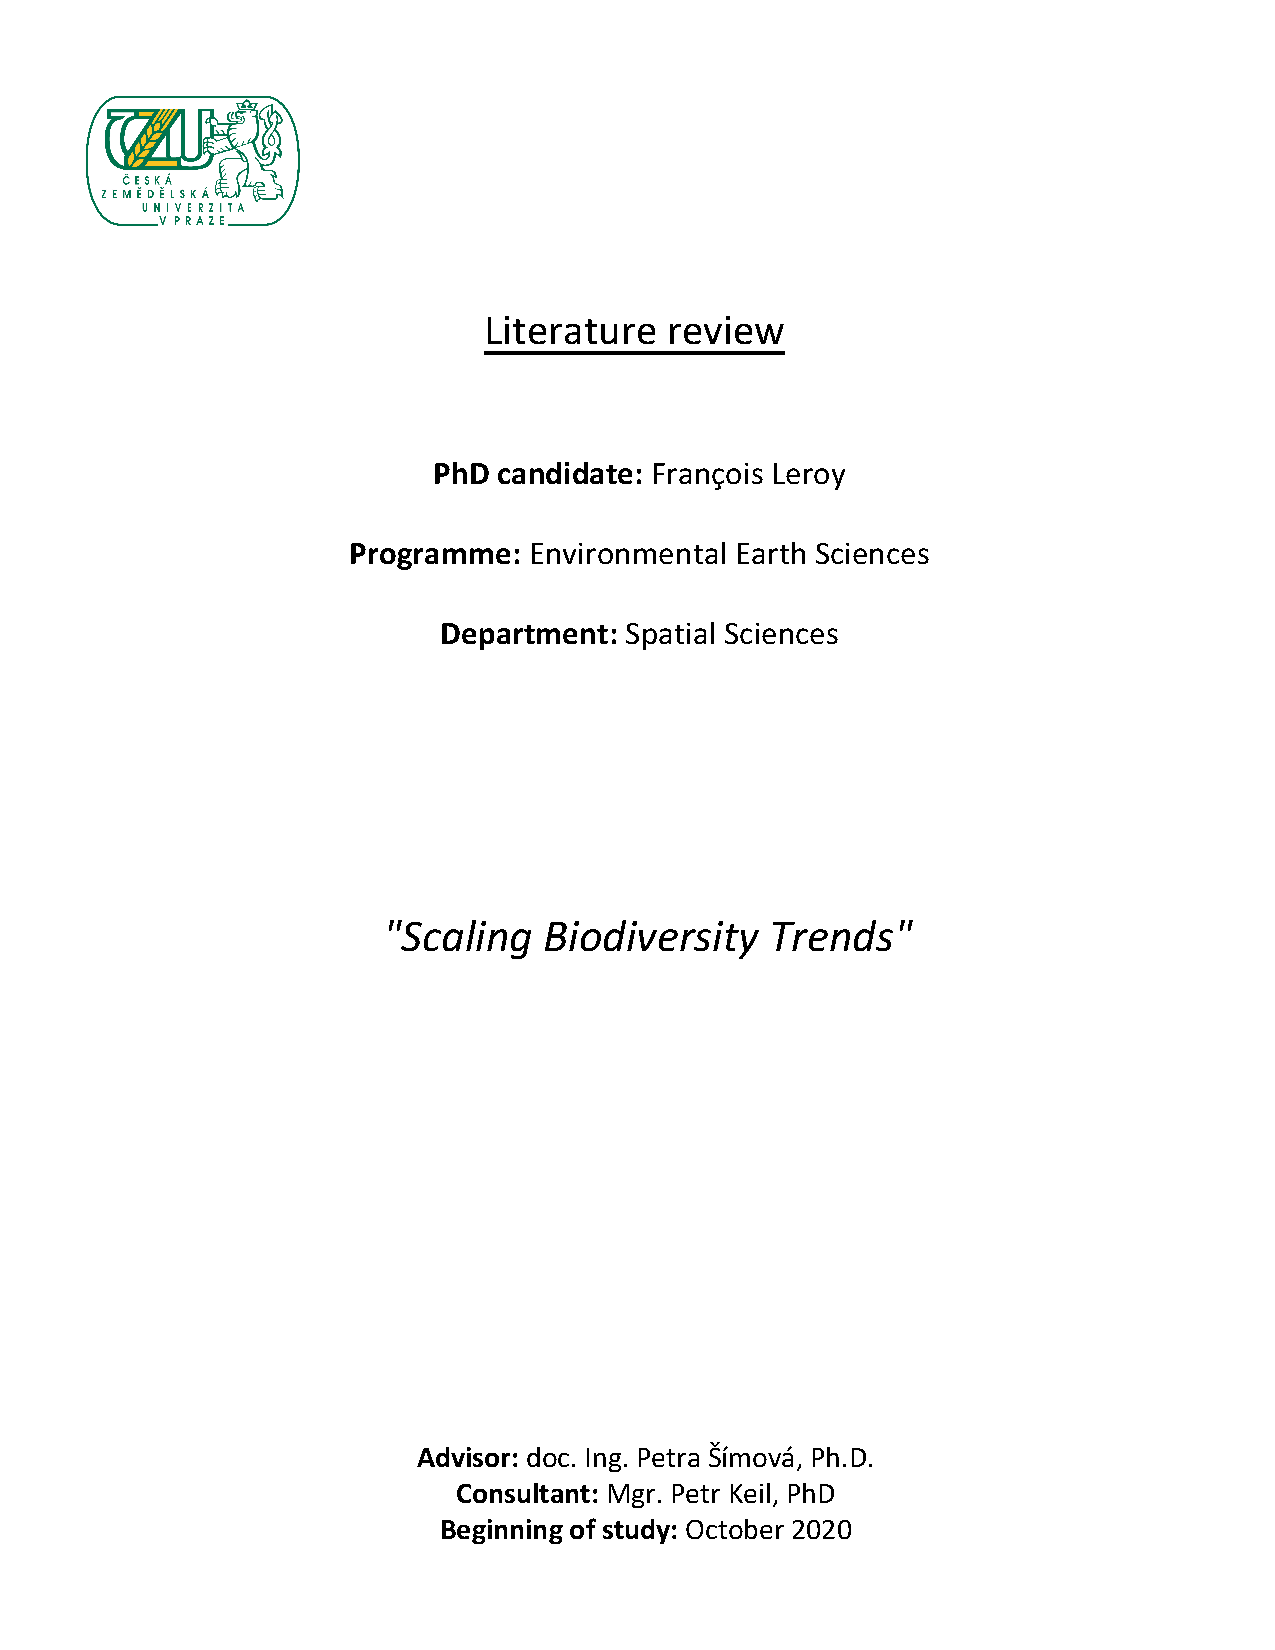
\includepdf[pages = {1}, fitpaper=true]{_assets/coverpage.pdf}

% Roman numbering for content before toc and toc itself
\cleardoublepage 
\pagenumbering{roman}

{
\hypersetup{linkcolor=}
\setcounter{tocdepth}{1}
\tableofcontents
\newpage
}
\vspace{50mm}
\setstretch{1.5}


% Start the arabic numbering at the 1st chapter
\cleardoublepage 
\pagenumbering{arabic}


% The mind, the...
\hypertarget{outline}{%
\chapter*{Outline}\label{outline}}
\addcontentsline{toc}{chapter}{Outline}

Literature review about the link between biodiversity facets trends and spatial/temporal scales.

The idea is to take every paper that talk about biodiversity trends (so far using just the species richness seems already a lot of paper) and to list \textbf{1)} which biodiversity metric they use \textbf{2)} which taxon/taxa they use, \textbf{3)} the spatial scale, \textbf{4)} the temporal scale and \textbf{5)} what is the dynamic (does the biodiversity metric increase/decrease/doesn't change over time/unclear).

Make a table of all these papers and \texttt{group\_by(taxa)\ \%\textgreater{}\%\ order\_by(spatial\_scale\ \textbar{}\ temporal\_scale)}. Then see if for each taxa we can find a trend (a bit like in Chase \emph{et al.} 2019 Oikos paper \textbar{} Jarzyna \emph{et al.} 2015 but here I am not making the analysis, just taking the analysis from papers). Best example found so far: \href{https://besjournals.onlinelibrary.wiley.com/doi/10.1111/j.0021-8901.2004.00926.x}{Hill \& Hamer 2004}

I am using the \enquote{Advanced Research} tab of Web of Science which allows me skim through the entire literature using a convenient syntax. For instance:

\begin{verbatim}
AB = ((biodiversity OR species richness OR diversity) AND
(temporal trend* OR dynamic*) AND
(bird* OR avia*)) 
\end{verbatim}

And

\begin{verbatim}
AB = ((biodiversity change index)  AND (bird*  OR avia*)  AND trend*)
\end{verbatim}

And

\begin{verbatim}
AB = ((species richness) AND (bird* OR avia*) AND trend*) 
\end{verbatim}

And

\begin{verbatim}
ALL=(birds AND species richness AND temporal trend)
\end{verbatim}

\hypertarget{dashboard}{%
\chapter*{Dashboard}\label{dashboard}}
\addcontentsline{toc}{chapter}{Dashboard}

\href{https://www.sciencedirect.com/science/article/pii/S1470160X20306658?via\%3Dihub}{Reference paper}

\begin{itemize}
\item
  05/07/2021: research wos made with the literature review filter for the first query (stopped at \#13) and created the second query (stopped at \#2)
\item
  07/07/2021: questions to Petr: \textbf{1)} can the geometric mean of relative abundance + the weighted goodness of fit be used as biodiversity trend index, \textbf{2)} can the Farmland Bird Indicator (FBI) be used as biodiversity trend (for me it is more biodiversity health, Chiron et al 2013) \textbf{3)} what about the Red List Index trend? \textbf{4)} what about Multispecies population indexes?
\item
  08/07/2021: stopped at the article 41 for research \#2.
\item
  12/08/2021: stopped at article 4 for research \#4
\item
  13/08/2021: stopped at article 8 for research \#4
\item
  17/08/2021: stopped at article 15 for research \#4
\item
  18/08/2021: stopped at article 30 for research \#4
\item
  19/08/2021: stopped at article 46 for research \#4
\item
  20/08/2021: stopped at article 64 for research \#4
\item
  01/09/2021: verifying spatial scales --\textgreater{} stopped at Dittrich 2019
\item
  02/09/2021: \textbf{Question 1:} for the FBI/WBI\ldots*BI indexes, usually they use a GLM/GAM to predict the abundance over the entire spatial extent and then compute the metric. Basically, those metrics are geometric means of predicted species abundances. Which spatial scale to use: the spatial unit of the prediction (i.e.~the plot), or the entire area predicted? (Imo, the second option is correct). \textbf{Question 2:} same question for the Geometric mean but I am realizing while writing this question that *BI are kind of similar to geometric means so answering the first question will answer this one.
\end{itemize}

\textbf{Papers that are driving me mad:} \citet{doxa_low-intensity_2010}, \citet{jiguet_french_2012}, and \citet{chiron_forecasting_2013}, \citet{eglington_disentangling_2012}

\hypertarget{introduction}{%
\chapter{Introduction}\label{introduction}}

Human life quality is intrinsically linked to ecosystems state that he is living in. Indeed, ecosystems services extend in a large spectrum of mechanisms including nutrient cycle, food production, or climate and water cycle regulation \citep{pereira_global_2012}. Some of those ecosystem functions are managed by bird biodiversity such as seed dispersal, controls pests or pollinate plant. Unfortunately, anthropogenic stressors like habitat loss, over exploitation, pollution or introduction of invasive species could lead biodiversity to its sixth mass extinction \citep{barnosky_has_2011}.

Biodiversity erosion is now known from everyone and political decisions has been stated in order to limit it \citep[\emph{e.g.}][2010, 2002]{the_convention_on_biological_diversity_convention_2021}. However, these objectives have been so far not reached due mainly to our confusion and misunderstanding about biodiversity dynamic and how to determine it.

As a matter of fact, studying biodiversity can be confusing, especially because several choices must be done. Firstly, the level at which you are looking at the biodiversity must be chosen (\emph{e.g.} species, functional, phylogenetic diversity). Secondly, one must decide which metric is the most appropriate for his study. There are many facets of biodiversity that can be measured by different metrics depending on the objective of your study. Measures of static biodiversity are commonly used such as species richness or \(\alpha\) diversity \citep[\emph{i.e.} number of species,][]{whittaker_vegetation_1960}, the Shannon index \citep{shannon_mathematical_1948} ,the Simpson index \citep{simpson_measurement_1949} or the Hill number \citep{hill_diversity_1973}. The later three biodiversity indexes take into account the relative abundances of the species and can be considered as the \emph{quality} of the biodiversity. On an other hand, the spatial and temporal \(\beta\) diversity will measure the species turnover and can be measured thanks to Whittaker's \citep{whittaker_evolution_1972}, Sørensen's \citep{sorensen_method_1948} or Jaccard's \citep{jaccard_distribution_1912} dissimilarity indexes \citep[\emph{e.g.}][]{keil_patterns_2012}.

However, overall biodiversity (\emph{i.e.} taking into account species of every taxa) may not be relevant for one's case study. Thus, several multi-species indicators have also been created, taking into account the abundances of indicator species giving information on the ecosystem health. The most known ones are the Red List Index \citep{butchart_improvements_2007, butchart_using_2005, butchart_measuring_2004} or the Biodiversity Change Index \citep{normander_indicator_2012}.

Using all the metrics cited above, we now know that the loss of global biodiversity is unprecedented. However, current scientific literature has also shown that temporal trends in local changes of biodiversity can be opposite to trends at larger scales \citep[\emph{e.g.}][]{chase_species_2019}. Thus, current changes in biodiversity is far more complex than a simple global decrease: most of the ecosystems undergo alterations of their communities with changes in species composition \citep{blowes_geography_2019, dornelas_quantifying_2013}. Wonders persist about how the trend of these different metrics of biodiversity are link to the spatial and temporal scales used when measured.

In order to investigate this link between spatial scales and biodiversity metrics, birds is a relevant taxon. Thanks to the many ornithological monitoring and surveys, we now have a large number of long, high-quality time series on bird populations \citep{bejcek_velke_2016}. Birds are easy to observe, easy to identify and thus many volunteers are motivated to conduct standardized sampling. Given their ability to change quickly of locations, their presence is also a good indicator for ecosystem health and thus several standardized metrics have been created to assess their populations. For instance, the geometric mean of relative abundances or the goodness-of-fit statistic \citep{studeny_goodness_2011} are some of the baseline. Other multi-species indicators have also been created specifically for birds, such as the Farmland Bird Indicator \citep{gregory_developing_2005}, the Forest Bird Indicator \citep{gregory_population_2007} or the Wild Bird Indicator \citep{gregory_wild_2010}.

Here, I propose to review articles assessing the temporal trends of different avian biodiversity metrics and to look at which spatial scales these studies have been done. Summarizing the trends of these qualitative and/or quantitative avian biodiversity indexes along with their spatial and temporal scales will help to see more clearly how the trends of biodiversity are linked to spatio-temporal scales. It is also important to demonstrate that the information about the sampling plan (\emph{i.e.} spatial scale, time span, temporal scales etc) is not systematically indicated in the scientific literature and can bring confusion to the analysis and comparisons of their trends. I believe that this review can help to have a better overview of the current knowledge on the trend of biodiversity metrics of bird populations.

\hypertarget{materials-and-methods}{%
\chapter{Materials and Methods}\label{materials-and-methods}}

For this review, articles of interest were the ones assessing temporal trends of the most common indicators (\emph{i.e.} metrics) of avian biodiversity and specifying spatial and temporal scales. For this, I used the \emph{\enquote{advanced search}} tool of the ISI Web of Science Core collection database with these four following queries:

\begin{enumerate}
\def\labelenumi{\arabic{enumi}.}
\item
  \texttt{AB\ =\ ((biodiversity\ OR\ species\ richness\ OR\ diversity)\ AND\ (temporal\ trend*\ OR\ dynamic*)\ AND\ (bird*\ OR\ avia*))} which resulted in 1346 references.
\item
  \texttt{AB\ =\ ((biodiversity\ change\ index)\ \ AND\ (bird*\ \ OR\ avia*)\ \ AND\ trend*)} which resulted in 60 references.
\item
  \texttt{AB\ =\ ((species\ richness)\ AND\ (bird*\ OR\ avia*)\ AND\ trend*)} which resulted in 313 references.
\item
  \texttt{ALL=(birds\ AND\ species\ richness\ AND\ temporal\ trend)} which resulted in 88 references.
\end{enumerate}

For each query, the title and abstract of the articles were reviewed. When the temporal trend was explicitly specified (either visually or literally), the material and method part was read in order to collect the \emph{spatial grain} of the trend (\emph{i.e.} the area at which the trend is assessed), its \emph{temporal grain} (\emph{i.e.} the time span at which data have been gathered on the field), the \emph{spatial extent} (\emph{i.e.} the entire area at which the study applies), the \emph{temporal extent} and the \emph{beginning and ending years} of the study as well as the \emph{general trend} of the metric (Tab. \ref{tab:maintable}).

Concerning the trend assessment, some papers contained the \emph{p-value} or directly specified the significant trend of the metric. However, a portion of papers gives only visual representations of the trend. For those, the standard error was used when displayed. For the very few only giving the trend, \textcolor{red}{the rule of thumb was applied}. Information can be found in the column \emph{Note} of the Tab. \ref{tab:notetable} of the supplementary material. Moreover, the final trend retained (\emph{i.e.} either \emph{Increase}, \emph{Stable} or \emph{Decrease}) doesn't reflect all the fluctuations of the metric through time but rather the difference between the starting and ending points.

Moreover, \citet{pilotto_meta-analysis_2020} conducted a meta-analysis in which they computed and summarized the trend of four biodiversity metrics (namely, species richness, species diversity, abundance and temporal turnover). Some of them were concerning bird communities. For those latter, I used their code and data on the \href{https://github.com/FrsLry/R-code}{github repository} of their paper in order to compute the trends of these four metrics for the bird datasets.

\begin{landscape}\begingroup\fontsize{10}{12}\selectfont

\begin{longtable}[t]{>{\raggedright\arraybackslash}p{6.5em}>{\raggedright\arraybackslash}p{6.5em}>{\raggedleft\arraybackslash}p{6.5em}>{\raggedleft\arraybackslash}p{6.5em}>{\raggedleft\arraybackslash}p{6.5em}>{\raggedleft\arraybackslash}p{6.5em}>{\raggedright\arraybackslash}p{6.5em}>{\raggedright\arraybackslash}p{6.5em}>{\raggedright\arraybackslash}p{6.5em}}
\caption{\label{tab:maintable}SR = species richness, Ab = abundance, Eve = evenness, }\\
\toprule
Reference & Metric & Spatial grain (Km²) & Temporal grain (year) & Spatial extent (Km²) & Temporal extent (year) & Years & Country & Trend\\
\midrule
\endfirsthead
\caption[]{\label{tab:maintable}SR = species richness, Ab = abundance, Eve = evenness,  \textit{(continued)}}\\
\toprule
Reference & Metric & Spatial grain (Km²) & Temporal grain (year) & Spatial extent (Km²) & Temporal extent (year) & Years & Country & Trend\\
\midrule
\endhead

\endfoot
\bottomrule
\endlastfoot
\cellcolor{gray!6}{\cite{barnagaud_temporal_2017}} & \cellcolor{gray!6}{SR} & \cellcolor{gray!6}{0.500} & \cellcolor{gray!6}{1.000} & \cellcolor{gray!6}{9834000.00} & \cellcolor{gray!6}{41} & \cellcolor{gray!6}{1970-2011} & \cellcolor{gray!6}{USA} & \cellcolor{gray!6}{Increase}\\
\cite{barnagaud_temporal_2017} & Abundance & 0.500 & 1.000 & 9834000.00 & 41 & 1970-2011 & USA & Decrease\\
\cellcolor{gray!6}{\cite{barnagaud_temporal_2017}} & \cellcolor{gray!6}{Evenness} & \cellcolor{gray!6}{0.500} & \cellcolor{gray!6}{1.000} & \cellcolor{gray!6}{9834000.00} & \cellcolor{gray!6}{41} & \cellcolor{gray!6}{1970-2011} & \cellcolor{gray!6}{USA} & \cellcolor{gray!6}{Increase}\\
\cite{barnagaud_temporal_2017} & Functional richness & 0.500 & 1.000 & 9834000.00 & 41 & 1970-2011 & USA & Increase\\
\cellcolor{gray!6}{\cite{barnagaud_temporal_2017}} & \cellcolor{gray!6}{Functional dispersion} & \cellcolor{gray!6}{0.500} & \cellcolor{gray!6}{1.000} & \cellcolor{gray!6}{9834000.00} & \cellcolor{gray!6}{41} & \cellcolor{gray!6}{1970-2011} & \cellcolor{gray!6}{USA} & \cellcolor{gray!6}{Stable}\\
\addlinespace
\cite{barnagaud_temporal_2017} & Functional evenness & 0.500 & 1.000 & 9834000.00 & 41 & 1970-2011 & USA & Increase\\
\cellcolor{gray!6}{\cite{roels_recovery_2019}} & \cellcolor{gray!6}{SR} & \cellcolor{gray!6}{0.040} & \cellcolor{gray!6}{1.000} & \cellcolor{gray!6}{0.04} & \cellcolor{gray!6}{5} & \cellcolor{gray!6}{NA} & \cellcolor{gray!6}{Panama} & \cellcolor{gray!6}{Increase}\\
\cite{roels_recovery_2019} & Bird activity & 0.040 & 1.000 & 0.04 & 5 & NA & Panama & Increase\\
\cellcolor{gray!6}{\cite{wretenberg_changes_2010}} & \cellcolor{gray!6}{SR} & \cellcolor{gray!6}{0.030} & \cellcolor{gray!6}{1.000} & \cellcolor{gray!6}{1800.00} & \cellcolor{gray!6}{11} & \cellcolor{gray!6}{1994-2004} & \cellcolor{gray!6}{Sweden} & \cellcolor{gray!6}{Decrease}\\
\cite{ram_what_2017} & SR & 1.600 & 1.000 & 350000.00 & 18 & 1998-2015 & Sweden & \vphantom{1} Increase\\
\addlinespace
\cellcolor{gray!6}{\cite{ram_what_2017}} & \cellcolor{gray!6}{SR} & \cellcolor{gray!6}{1.600} & \cellcolor{gray!6}{1.000} & \cellcolor{gray!6}{350000.00} & \cellcolor{gray!6}{18} & \cellcolor{gray!6}{1998-2015} & \cellcolor{gray!6}{Sweden} & \cellcolor{gray!6}{Stable}\\
\cite{ram_what_2017} & SR & 1.600 & 1.000 & 350000.00 & 18 & 1998-2015 & Sweden & Increase\\
\cellcolor{gray!6}{\cite{ram_what_2017}} & \cellcolor{gray!6}{Multi-species indicator} & \cellcolor{gray!6}{1.600} & \cellcolor{gray!6}{1.000} & \cellcolor{gray!6}{350000.00} & \cellcolor{gray!6}{18} & \cellcolor{gray!6}{1998-2015} & \cellcolor{gray!6}{Sweden} & \cellcolor{gray!6}{\vphantom{1} Increase}\\
\cite{ram_what_2017} & Multi-species indicator & 1.600 & 1.000 & 350000.00 & 18 & 1998-2015 & Sweden & Increase\\
\cellcolor{gray!6}{\cite{harrison_quantifying_2016}} & \cellcolor{gray!6}{Geometric mean} & \cellcolor{gray!6}{10000.000} & \cellcolor{gray!6}{0.500} & \cellcolor{gray!6}{NA} & \cellcolor{gray!6}{20} & \cellcolor{gray!6}{1994-2013} & \cellcolor{gray!6}{UK} & \cellcolor{gray!6}{Increase}\\
\addlinespace
\cite{harrison_quantifying_2016} & GoF ( $\lambda$ = -1) & 10000.000 & 0.500 & NA & 20 & 1994-2013 & UK & Stable\\
\cellcolor{gray!6}{\cite{harrison_quantifying_2016}} & \cellcolor{gray!6}{GoF ( $\lambda$ = -2)} & \cellcolor{gray!6}{10000.000} & \cellcolor{gray!6}{0.500} & \cellcolor{gray!6}{NA} & \cellcolor{gray!6}{20} & \cellcolor{gray!6}{1994-2013} & \cellcolor{gray!6}{UK} & \cellcolor{gray!6}{Stable}\\
\cite{doxa_low-intensity_2010} & FBI & 4.000 & 1.000 & 643801.00 & 8 & 2001-2008 & France & Increase\\
\cellcolor{gray!6}{\cite{doxa_low-intensity_2010}} & \cellcolor{gray!6}{FBI} & \cellcolor{gray!6}{4.000} & \cellcolor{gray!6}{1.000} & \cellcolor{gray!6}{643801.00} & \cellcolor{gray!6}{8} & \cellcolor{gray!6}{2001-2008} & \cellcolor{gray!6}{France} & \cellcolor{gray!6}{\vphantom{1} Stable}\\
\cite{doxa_low-intensity_2010} & FBI & 4.000 & 1.000 & 643801.00 & 8 & 2001-2008 & France & Stable\\
\addlinespace
\cellcolor{gray!6}{\cite{arnold_contrasting_2021}} & \cellcolor{gray!6}{SR} & \cellcolor{gray!6}{0.020} & \cellcolor{gray!6}{1.000} & \cellcolor{gray!6}{1000.00} & \cellcolor{gray!6}{100} & \cellcolor{gray!6}{NA} & \cellcolor{gray!6}{Trinidad} & \cellcolor{gray!6}{Stable}\\
\cite{arnold_contrasting_2021} & Shannon & 0.020 & 1.000 & 1000.00 & 100 & NA & Trinidad & Stable\\
\cellcolor{gray!6}{\cite{arnold_contrasting_2021}} & \cellcolor{gray!6}{Simpson} & \cellcolor{gray!6}{0.020} & \cellcolor{gray!6}{1.000} & \cellcolor{gray!6}{1000.00} & \cellcolor{gray!6}{100} & \cellcolor{gray!6}{NA} & \cellcolor{gray!6}{Trinidad} & \cellcolor{gray!6}{Stable}\\
\cite{xu_detecting_2018} & SR & 6.560 & 1.000 & 6.56 & 12 & 2002-2013 & China & Decrease\\
\cellcolor{gray!6}{\cite{jiguet_french_2012}} & \cellcolor{gray!6}{GBI} & \cellcolor{gray!6}{4.000} & \cellcolor{gray!6}{1.000} & \cellcolor{gray!6}{643801.00} & \cellcolor{gray!6}{22} & \cellcolor{gray!6}{1989-2009} & \cellcolor{gray!6}{France} & \cellcolor{gray!6}{Increase}\\
\addlinespace
\cite{jiguet_french_2012} & WBI & 4.000 & 1.000 & 643801.00 & 22 & 1989-2009 & France & Increase\\
\cellcolor{gray!6}{\cite{jiguet_french_2012}} & \cellcolor{gray!6}{UBI} & \cellcolor{gray!6}{4.000} & \cellcolor{gray!6}{1.000} & \cellcolor{gray!6}{643801.00} & \cellcolor{gray!6}{22} & \cellcolor{gray!6}{1989-2009} & \cellcolor{gray!6}{France} & \cellcolor{gray!6}{Increase}\\
\cite{jiguet_french_2012} & FBI & 4.000 & 1.000 & 643801.00 & 22 & 1989-2009 & France & Increase\\
\cellcolor{gray!6}{\cite{jiguet_french_2012}} & \cellcolor{gray!6}{EU bird directive} & \cellcolor{gray!6}{4.000} & \cellcolor{gray!6}{1.000} & \cellcolor{gray!6}{643801.00} & \cellcolor{gray!6}{22} & \cellcolor{gray!6}{1989-2009} & \cellcolor{gray!6}{France} & \cellcolor{gray!6}{Increase}\\
\cite{jiguet_french_2012} & RLI (Red list Index) & NA & 1.000 & 10180000.00 & 22 & 1989-2009 & France & Decrease\\
\addlinespace
\cellcolor{gray!6}{\cite{keten_temporal_nodate}} & \cellcolor{gray!6}{SR} & \cellcolor{gray!6}{1.700} & \cellcolor{gray!6}{1.000} & \cellcolor{gray!6}{1.70} & \cellcolor{gray!6}{11} & \cellcolor{gray!6}{2006-2016} & \cellcolor{gray!6}{Turkey} & \cellcolor{gray!6}{Stable}\\
\cite{davey_rise_2012} & Simpson & 1.000 & 1.000 & 242495.00 & 13 & 1994-2006 & UK & Increase\\
\cellcolor{gray!6}{\cite{davey_rise_2012}} & \cellcolor{gray!6}{SR} & \cellcolor{gray!6}{1.000} & \cellcolor{gray!6}{1.000} & \cellcolor{gray!6}{242495.00} & \cellcolor{gray!6}{13} & \cellcolor{gray!6}{1994-2006} & \cellcolor{gray!6}{UK} & \cellcolor{gray!6}{Increase}\\
\cite{davey_rise_2012} & Evenness & 1.000 & 1.000 & 242495.00 & 13 & 1994-2006 & UK & Increase\\
\cellcolor{gray!6}{\cite{christian_more_2009}} & \cellcolor{gray!6}{SR} & \cellcolor{gray!6}{15.400} & \cellcolor{gray!6}{NA} & \cellcolor{gray!6}{15.40} & \cellcolor{gray!6}{209} & \cellcolor{gray!6}{1898-2006} & \cellcolor{gray!6}{France} & \cellcolor{gray!6}{Increase}\\
\addlinespace
\cite{dittrich_multiyear_2019} & SR & 0.053 & 0.330 & 53.00 & 3 & 2010-2012 & Spain & Increase\\
\cellcolor{gray!6}{\cite{dittrich_multiyear_2019}} & \cellcolor{gray!6}{SR} & \cellcolor{gray!6}{0.053} & \cellcolor{gray!6}{1.000} & \cellcolor{gray!6}{53.00} & \cellcolor{gray!6}{3} & \cellcolor{gray!6}{2010-2012} & \cellcolor{gray!6}{Spain} & \cellcolor{gray!6}{Increase}\\
\cite{dittrich_multiyear_2019} & SR & 0.083 & 0.330 & 53.00 & 3 & 2012-2014 & UK & Stable\\
\cellcolor{gray!6}{\cite{dittrich_multiyear_2019}} & \cellcolor{gray!6}{SR} & \cellcolor{gray!6}{0.083} & \cellcolor{gray!6}{1.000} & \cellcolor{gray!6}{53.00} & \cellcolor{gray!6}{3} & \cellcolor{gray!6}{2012-2014} & \cellcolor{gray!6}{UK} & \cellcolor{gray!6}{Stable}\\
\cite{sirami_changes_2012} & SR & 0.380 & 1.000 & 430.00 & 21 & 1998-2018 & Swaziland & Decrease\\
\addlinespace
\cellcolor{gray!6}{\cite{garcia-navas_temporal_2020}} & \cellcolor{gray!6}{Spatial beta-diversity} & \cellcolor{gray!6}{267.000} & \cellcolor{gray!6}{1.000} & \cellcolor{gray!6}{267.00} & \cellcolor{gray!6}{20} & \cellcolor{gray!6}{1999-2018} & \cellcolor{gray!6}{Switzerland} & \cellcolor{gray!6}{Decrease}\\
\cite{ellis_twenty-year_2019} & SR & 0.160 & 1.000 & NA & 21 & 1994-2014 & Oregon, USA & \vphantom{1} Stable\\
\cellcolor{gray!6}{\cite{ellis_twenty-year_2019}} & \cellcolor{gray!6}{SR} & \cellcolor{gray!6}{0.160} & \cellcolor{gray!6}{1.000} & \cellcolor{gray!6}{NA} & \cellcolor{gray!6}{21} & \cellcolor{gray!6}{1994-2014} & \cellcolor{gray!6}{Oregon, USA} & \cellcolor{gray!6}{Stable}\\
\cite{ellis_twenty-year_2019} & SR & 0.160 & 1.000 & NA & 21 & 1994-2014 & Oregon, USA & Increase\\
\cellcolor{gray!6}{\cite{ellis_twenty-year_2019}} & \cellcolor{gray!6}{SR} & \cellcolor{gray!6}{0.480} & \cellcolor{gray!6}{1.000} & \cellcolor{gray!6}{NA} & \cellcolor{gray!6}{21} & \cellcolor{gray!6}{1994-2014} & \cellcolor{gray!6}{Oregon, USA} & \cellcolor{gray!6}{Stable}\\
\addlinespace
\cite{ellis_twenty-year_2019} & Shannon & 0.160 & 1.000 & NA & 21 & 1994-2014 & Oregon, USA & \vphantom{1} Increase\\
\cellcolor{gray!6}{\cite{ellis_twenty-year_2019}} & \cellcolor{gray!6}{Shannon} & \cellcolor{gray!6}{0.160} & \cellcolor{gray!6}{1.000} & \cellcolor{gray!6}{NA} & \cellcolor{gray!6}{21} & \cellcolor{gray!6}{1994-2014} & \cellcolor{gray!6}{Oregon, USA} & \cellcolor{gray!6}{Decrease}\\
\cite{ellis_twenty-year_2019} & Shannon & 0.160 & 1.000 & NA & 21 & 1994-2014 & Oregon, USA & Increase\\
\cellcolor{gray!6}{\cite{ellis_twenty-year_2019}} & \cellcolor{gray!6}{Shannon} & \cellcolor{gray!6}{0.480} & \cellcolor{gray!6}{1.000} & \cellcolor{gray!6}{NA} & \cellcolor{gray!6}{21} & \cellcolor{gray!6}{1994-2014} & \cellcolor{gray!6}{Oregon, USA} & \cellcolor{gray!6}{Increase}\\
\cite{ellis_twenty-year_2019} & Simpson & 0.160 & 1.000 & NA & 21 & 1994-2014 & Oregon, USA & \vphantom{1} Increase\\
\addlinespace
\cellcolor{gray!6}{\cite{ellis_twenty-year_2019}} & \cellcolor{gray!6}{Simpson} & \cellcolor{gray!6}{0.160} & \cellcolor{gray!6}{1.000} & \cellcolor{gray!6}{NA} & \cellcolor{gray!6}{21} & \cellcolor{gray!6}{1994-2014} & \cellcolor{gray!6}{Oregon, USA} & \cellcolor{gray!6}{Decrease}\\
\cite{ellis_twenty-year_2019} & Simpson & 0.160 & 1.000 & NA & 21 & 1994-2014 & Oregon, USA & Increase\\
\cellcolor{gray!6}{\cite{ellis_twenty-year_2019}} & \cellcolor{gray!6}{Simpson} & \cellcolor{gray!6}{0.480} & \cellcolor{gray!6}{1.000} & \cellcolor{gray!6}{NA} & \cellcolor{gray!6}{21} & \cellcolor{gray!6}{1994-2014} & \cellcolor{gray!6}{Oregon, USA} & \cellcolor{gray!6}{Decrease}\\
\cite{sicurella_effectiveness_2018} & Occurence (\%) & 17370.300 & 1.000 & 23844.00 & 22 & 1992-2013 & Lombardy, Italy & Stable\\
\cellcolor{gray!6}{\cite{sicurella_effectiveness_2018}} & \cellcolor{gray!6}{Occurence (\%)} & \cellcolor{gray!6}{1403.900} & \cellcolor{gray!6}{1.000} & \cellcolor{gray!6}{23844.00} & \cellcolor{gray!6}{22} & \cellcolor{gray!6}{1992-2013} & \cellcolor{gray!6}{Lombardy, Italy} & \cellcolor{gray!6}{Stable}\\
\addlinespace
\cite{sicurella_effectiveness_2018} & Occurence (\%) & 6461.900 & 1.000 & 23844.00 & 22 & 1992-2013 & Lombardy, Italy & Increase\\
\cellcolor{gray!6}{\cite{nally_monitoring_1997}} & \cellcolor{gray!6}{SR} & \cellcolor{gray!6}{0.490} & \cellcolor{gray!6}{0.003} & \cellcolor{gray!6}{10.00} & \cellcolor{gray!6}{3} & \cellcolor{gray!6}{1994-1996} & \cellcolor{gray!6}{Australia} & \cellcolor{gray!6}{Increase}\\
\cite{latta_patterns_2011} & SR & 1.180 & 2.000 & NA & 14 & 1994-2007 & Ecuador & \vphantom{1} Decrease\\
\cellcolor{gray!6}{\cite{latta_patterns_2011}} & \cellcolor{gray!6}{SR} & \cellcolor{gray!6}{1.180} & \cellcolor{gray!6}{2.000} & \cellcolor{gray!6}{NA} & \cellcolor{gray!6}{14} & \cellcolor{gray!6}{1994-2007} & \cellcolor{gray!6}{Ecuador} & \cellcolor{gray!6}{Decrease}\\
\cite{scarton_long-term_2017} & SR & 0.550 & 2.000 & 0.55 & 25 & 1990-2014 & Lagoon of Venice, Italy & Increase\\
\addlinespace
\cellcolor{gray!6}{\cite{scarton_long-term_2017}} & \cellcolor{gray!6}{Shannon} & \cellcolor{gray!6}{0.550} & \cellcolor{gray!6}{2.000} & \cellcolor{gray!6}{0.55} & \cellcolor{gray!6}{25} & \cellcolor{gray!6}{1990-2014} & \cellcolor{gray!6}{Lagoon of Venice, Italy} & \cellcolor{gray!6}{Increase}\\
\cite{scarton_long-term_2017} & Temporal beta-diversity & 0.550 & 2.000 & 0.55 & 25 & 1990-2014 & Lagoon of Venice, Italy & \vphantom{1} Increase\\
\cellcolor{gray!6}{\cite{scarton_long-term_2017}} & \cellcolor{gray!6}{Temporal beta-diversity} & \cellcolor{gray!6}{0.550} & \cellcolor{gray!6}{2.000} & \cellcolor{gray!6}{0.55} & \cellcolor{gray!6}{25} & \cellcolor{gray!6}{1990-2014} & \cellcolor{gray!6}{Lagoon of Venice, Italy} & \cellcolor{gray!6}{Increase}\\
\cite{chiron_forecasting_2013} & FBI & 4.000 & 1.000 & 643801.00 & 14 & 2007-2020 & France & \vphantom{3} Decrease\\
\cellcolor{gray!6}{\cite{chiron_forecasting_2013}} & \cellcolor{gray!6}{FBI} & \cellcolor{gray!6}{4.000} & \cellcolor{gray!6}{1.000} & \cellcolor{gray!6}{643801.00} & \cellcolor{gray!6}{14} & \cellcolor{gray!6}{2007-2020} & \cellcolor{gray!6}{France} & \cellcolor{gray!6}{\vphantom{2} Decrease}\\
\addlinespace
\cite{chiron_forecasting_2013} & FBI & 4.000 & 1.000 & 643801.00 & 14 & 2007-2020 & France & \vphantom{1} Decrease\\
\cellcolor{gray!6}{\cite{chiron_forecasting_2013}} & \cellcolor{gray!6}{FBI} & \cellcolor{gray!6}{4.000} & \cellcolor{gray!6}{1.000} & \cellcolor{gray!6}{643801.00} & \cellcolor{gray!6}{14} & \cellcolor{gray!6}{2007-2020} & \cellcolor{gray!6}{France} & \cellcolor{gray!6}{Decrease}\\
\cite{eglington_disentangling_2012} & FBI & 1.000 & 1.000 & 242495.00 & 39 & 1970-2008 & UK & Decrease\\
\cellcolor{gray!6}{\cite{harrison_assessing_2014}} & \cellcolor{gray!6}{Geometric mean} & \cellcolor{gray!6}{10000.000} & \cellcolor{gray!6}{1.000} & \cellcolor{gray!6}{200000.00} & \cellcolor{gray!6}{18} & \cellcolor{gray!6}{1994-2011} & \cellcolor{gray!6}{Great Britain, UK} & \cellcolor{gray!6}{Stable}\\
\cite{harrison_assessing_2014} & GoF ( $\lambda$ = -1) & 10000.000 & 1.000 & 200000.00 & 18 & 1994-2011 & Great Britain, UK & Decrease\\
\addlinespace
\cellcolor{gray!6}{\cite{harrison_assessing_2014}} & \cellcolor{gray!6}{GoF ( $\lambda$ = -2)} & \cellcolor{gray!6}{10000.000} & \cellcolor{gray!6}{1.000} & \cellcolor{gray!6}{200000.00} & \cellcolor{gray!6}{18} & \cellcolor{gray!6}{1994-2011} & \cellcolor{gray!6}{Great Britain, UK} & \cellcolor{gray!6}{Increase}\\
\cite{harrison_assessing_2014} & Geometric mean & 62000.000 & 1.000 & 77933.00 & 18 & 1994-2011 & Scotland, UK & Increase\\
\cellcolor{gray!6}{\cite{harrison_assessing_2014}} & \cellcolor{gray!6}{GoF ( $\lambda$ = -1)} & \cellcolor{gray!6}{62000.000} & \cellcolor{gray!6}{1.000} & \cellcolor{gray!6}{77933.00} & \cellcolor{gray!6}{18} & \cellcolor{gray!6}{1994-2011} & \cellcolor{gray!6}{Scotland, UK} & \cellcolor{gray!6}{Stable}\\
\cite{harrison_assessing_2014} & GoF ( $\lambda$ = -2) & 62000.000 & 1.000 & 77933.00 & 18 & 1994-2011 & Scotland, UK & Increase\\
\cellcolor{gray!6}{\cite{harrison_assessing_2014}} & \cellcolor{gray!6}{Geometric mean} & \cellcolor{gray!6}{16000.000} & \cellcolor{gray!6}{1.000} & \cellcolor{gray!6}{20779.00} & \cellcolor{gray!6}{18} & \cellcolor{gray!6}{1994-2011} & \cellcolor{gray!6}{Wales, UK} & \cellcolor{gray!6}{Stable}\\
\addlinespace
\cite{harrison_assessing_2014} & GoF ( $\lambda$ = -1) & 16000.000 & 1.000 & 20779.00 & 18 & 1994-2011 & Wales, UK & Stable\\
\cellcolor{gray!6}{\cite{harrison_assessing_2014}} & \cellcolor{gray!6}{GoF ( $\lambda$ = -2)} & \cellcolor{gray!6}{16000.000} & \cellcolor{gray!6}{1.000} & \cellcolor{gray!6}{20779.00} & \cellcolor{gray!6}{18} & \cellcolor{gray!6}{1994-2011} & \cellcolor{gray!6}{Wales, UK} & \cellcolor{gray!6}{Stable}\\
\cite{harrison_assessing_2014} & Geometric mean & 130000.000 & 1.000 & 130279.00 & 18 & 1994-2011 & England, UK & Decrease\\
\cellcolor{gray!6}{\cite{harrison_assessing_2014}} & \cellcolor{gray!6}{GoF ( $\lambda$ = -1)} & \cellcolor{gray!6}{130000.000} & \cellcolor{gray!6}{1.000} & \cellcolor{gray!6}{130279.00} & \cellcolor{gray!6}{18} & \cellcolor{gray!6}{1994-2011} & \cellcolor{gray!6}{England, UK} & \cellcolor{gray!6}{Decrease}\\
\cite{harrison_assessing_2014} & GoF ( $\lambda$ = -2) & 130000.000 & 1.000 & 130279.00 & 18 & 1994-2011 & England, UK & Stable\\
\addlinespace
\cellcolor{gray!6}{\cite{harrison_assessing_2014}} & \cellcolor{gray!6}{Geometric mean} & \cellcolor{gray!6}{10000.000} & \cellcolor{gray!6}{1.000} & \cellcolor{gray!6}{200000.00} & \cellcolor{gray!6}{18} & \cellcolor{gray!6}{1994-2011} & \cellcolor{gray!6}{Great Britain, UK} & \cellcolor{gray!6}{Increase}\\
\cite{harrison_assessing_2014} & GoF ( $\lambda$ = -1) & 10000.000 & 1.000 & 200000.00 & 18 & 1994-2011 & Great Britain, UK & Stable\\
\cellcolor{gray!6}{\cite{harrison_assessing_2014}} & \cellcolor{gray!6}{GoF ( $\lambda$ = -2)} & \cellcolor{gray!6}{10000.000} & \cellcolor{gray!6}{1.000} & \cellcolor{gray!6}{200000.00} & \cellcolor{gray!6}{18} & \cellcolor{gray!6}{1994-2011} & \cellcolor{gray!6}{Great Britain, UK} & \cellcolor{gray!6}{Decrease}\\
\cite{harrison_assessing_2014} & Geometric mean & 14000.000 & 1.000 & 77933.00 & 18 & 1994-2011 & Scotland, UK & Increase\\
\cellcolor{gray!6}{\cite{harrison_assessing_2014}} & \cellcolor{gray!6}{GoF ( $\lambda$ = -1)} & \cellcolor{gray!6}{14000.000} & \cellcolor{gray!6}{1.000} & \cellcolor{gray!6}{77933.00} & \cellcolor{gray!6}{18} & \cellcolor{gray!6}{1994-2011} & \cellcolor{gray!6}{Scotland, UK} & \cellcolor{gray!6}{Increase}\\
\addlinespace
\cite{harrison_assessing_2014} & GoF ( $\lambda$ = -2) & 14000.000 & 1.000 & 77933.00 & 18 & 1994-2011 & Scotland, UK & Stable\\
\cellcolor{gray!6}{\cite{harrison_assessing_2014}} & \cellcolor{gray!6}{Geometric mean} & \cellcolor{gray!6}{32300.000} & \cellcolor{gray!6}{1.000} & \cellcolor{gray!6}{130279.00} & \cellcolor{gray!6}{18} & \cellcolor{gray!6}{1994-2011} & \cellcolor{gray!6}{England, UK} & \cellcolor{gray!6}{Increase}\\
\cite{harrison_assessing_2014} & GoF ( $\lambda$ = -1) & 32300.000 & 1.000 & 130279.00 & 18 & 1994-2011 & England, UK & Decrease\\
\cellcolor{gray!6}{\cite{harrison_assessing_2014}} & \cellcolor{gray!6}{GoF ( $\lambda$ = -2)} & \cellcolor{gray!6}{32300.000} & \cellcolor{gray!6}{1.000} & \cellcolor{gray!6}{130279.00} & \cellcolor{gray!6}{18} & \cellcolor{gray!6}{1994-2011} & \cellcolor{gray!6}{England, UK} & \cellcolor{gray!6}{Stable}\\
\cite{harrison_assessing_2014} & Geometric mean & 3116.000 & 1.000 & 20779.00 & 18 & 1994-2011 & Wales, UK & Stable\\
\addlinespace
\cellcolor{gray!6}{\cite{harrison_assessing_2014}} & \cellcolor{gray!6}{GoF ( $\lambda$ = -1)} & \cellcolor{gray!6}{3116.000} & \cellcolor{gray!6}{1.000} & \cellcolor{gray!6}{20779.00} & \cellcolor{gray!6}{18} & \cellcolor{gray!6}{1994-2011} & \cellcolor{gray!6}{Wales, UK} & \cellcolor{gray!6}{Stable}\\
\cite{harrison_assessing_2014} & GoF ( $\lambda$ = -2) & 3116.000 & 1.000 & 20779.00 & 18 & 1994-2011 & Wales, UK & Increase\\
\cellcolor{gray!6}{\cite{juslen_application_2013}} & \cellcolor{gray!6}{RLI (Red list Index)} & \cellcolor{gray!6}{338440.000} & \cellcolor{gray!6}{1.000} & \cellcolor{gray!6}{338440.00} & \cellcolor{gray!6}{10} & \cellcolor{gray!6}{2001-2010} & \cellcolor{gray!6}{Finland} & \cellcolor{gray!6}{Decrease}\\
\cite{normander_indicator_2012} & BCI (Biodviersity Change Index) & 84266.000 & NA & 1260663.00 & 16 & 1990-2005 & Finland, Sweden, Norway, Denmark and Iceland & Decrease\\
\cellcolor{gray!6}{\cite{normander_indicator_2012}} & \cellcolor{gray!6}{BCI (Biodviersity Change Index)} & \cellcolor{gray!6}{529831.000} & \cellcolor{gray!6}{NA} & \cellcolor{gray!6}{1260663.00} & \cellcolor{gray!6}{16} & \cellcolor{gray!6}{1990-2005} & \cellcolor{gray!6}{Finland, Sweden, Norway, Denmark and Iceland} & \cellcolor{gray!6}{Stable}\\
\addlinespace
\cite{normander_indicator_2012} & BCI (Biodviersity Change Index) & 163131.000 & NA & 1260663.00 & 16 & 1990-2005 & Finland, Sweden, Norway, Denmark and Iceland & Decrease\\
\cellcolor{gray!6}{\cite{schipper_contrasting_2016}} & \cellcolor{gray!6}{Geometric mean} & \cellcolor{gray!6}{32.000} & \cellcolor{gray!6}{5.000} & \cellcolor{gray!6}{21792000.00} & \cellcolor{gray!6}{40} & \cellcolor{gray!6}{1971-2010} & \cellcolor{gray!6}{Canada, USA, Mexico} & \cellcolor{gray!6}{\vphantom{1} Increase}\\
\cite{schipper_contrasting_2016} & Geometric mean & 32.000 & 5.000 & 21792000.00 & 40 & 1971-2010 & Canada, USA, Mexico & Decrease\\
\cellcolor{gray!6}{\cite{schipper_contrasting_2016}} & \cellcolor{gray!6}{Geometric mean} & \cellcolor{gray!6}{32.000} & \cellcolor{gray!6}{5.000} & \cellcolor{gray!6}{21792000.00} & \cellcolor{gray!6}{40} & \cellcolor{gray!6}{1971-2010} & \cellcolor{gray!6}{Canada, USA, Mexico} & \cellcolor{gray!6}{Increase}\\
\cite{schipper_contrasting_2016} & Geometric mean & 32.000 & 5.000 & 22792000.00 & 40 & 1971-2010 & Canada, USA, Mexico & Increase\\
\addlinespace
\cellcolor{gray!6}{\cite{schipper_contrasting_2016}} & \cellcolor{gray!6}{Geometric mean} & \cellcolor{gray!6}{32.000} & \cellcolor{gray!6}{5.000} & \cellcolor{gray!6}{23792000.00} & \cellcolor{gray!6}{40} & \cellcolor{gray!6}{1971-2010} & \cellcolor{gray!6}{Canada, USA, Mexico} & \cellcolor{gray!6}{Stable}\\
\cite{schipper_contrasting_2016} & SR & 32.000 & 5.000 & 24792000.00 & 40 & 1971-2010 & Canada, USA, Mexico & Increase\\
\cellcolor{gray!6}{\cite{schipper_contrasting_2016}} & \cellcolor{gray!6}{SR} & \cellcolor{gray!6}{32.000} & \cellcolor{gray!6}{5.000} & \cellcolor{gray!6}{25792000.00} & \cellcolor{gray!6}{40} & \cellcolor{gray!6}{1971-2010} & \cellcolor{gray!6}{Canada, USA, Mexico} & \cellcolor{gray!6}{Decrease}\\
\cite{schipper_contrasting_2016} & SR & 32.000 & 5.000 & 26792000.00 & 40 & 1971-2010 & Canada, USA, Mexico & Increase\\
\cellcolor{gray!6}{\cite{schipper_contrasting_2016}} & \cellcolor{gray!6}{SR} & \cellcolor{gray!6}{32.000} & \cellcolor{gray!6}{5.000} & \cellcolor{gray!6}{27792000.00} & \cellcolor{gray!6}{40} & \cellcolor{gray!6}{1971-2010} & \cellcolor{gray!6}{Canada, USA, Mexico} & \cellcolor{gray!6}{Increase}\\
\addlinespace
\cite{schipper_contrasting_2016} & SR & 32.000 & 5.000 & 28792000.00 & 40 & 1971-2010 & Canada, USA, Mexico & Stable\\
\cellcolor{gray!6}{\cite{schipper_contrasting_2016}} & \cellcolor{gray!6}{Shannon} & \cellcolor{gray!6}{32.000} & \cellcolor{gray!6}{5.000} & \cellcolor{gray!6}{29792000.00} & \cellcolor{gray!6}{40} & \cellcolor{gray!6}{1971-2010} & \cellcolor{gray!6}{Canada, USA, Mexico} & \cellcolor{gray!6}{Increase}\\
\cite{schipper_contrasting_2016} & Shannon & 32.000 & 5.000 & 30792000.00 & 40 & 1971-2010 & Canada, USA, Mexico & Decrease\\
\cellcolor{gray!6}{\cite{schipper_contrasting_2016}} & \cellcolor{gray!6}{Shannon} & \cellcolor{gray!6}{32.000} & \cellcolor{gray!6}{5.000} & \cellcolor{gray!6}{31792000.00} & \cellcolor{gray!6}{40} & \cellcolor{gray!6}{1971-2010} & \cellcolor{gray!6}{Canada, USA, Mexico} & \cellcolor{gray!6}{Increase}\\
\cite{schipper_contrasting_2016} & Shannon & 32.000 & 5.000 & 32792000.00 & 40 & 1971-2010 & Canada, USA, Mexico & Increase\\
\addlinespace
\cellcolor{gray!6}{\cite{schipper_contrasting_2016}} & \cellcolor{gray!6}{Shannon} & \cellcolor{gray!6}{32.000} & \cellcolor{gray!6}{5.000} & \cellcolor{gray!6}{33792000.00} & \cellcolor{gray!6}{40} & \cellcolor{gray!6}{1971-2010} & \cellcolor{gray!6}{Canada, USA, Mexico} & \cellcolor{gray!6}{Increase}\\
\cite{schipper_contrasting_2016} & Simpson & 32.000 & 5.000 & 34792000.00 & 40 & 1971-2010 & Canada, USA, Mexico & Increase\\
\cellcolor{gray!6}{\cite{schipper_contrasting_2016}} & \cellcolor{gray!6}{Simpson} & \cellcolor{gray!6}{32.000} & \cellcolor{gray!6}{5.000} & \cellcolor{gray!6}{35792000.00} & \cellcolor{gray!6}{40} & \cellcolor{gray!6}{1971-2010} & \cellcolor{gray!6}{Canada, USA, Mexico} & \cellcolor{gray!6}{Stable}\\
\cite{schipper_contrasting_2016} & Simpson & 32.000 & 5.000 & 36792000.00 & 40 & 1971-2010 & Canada, USA, Mexico & Increase\\
\cellcolor{gray!6}{\cite{schipper_contrasting_2016}} & \cellcolor{gray!6}{Simpson} & \cellcolor{gray!6}{32.000} & \cellcolor{gray!6}{5.000} & \cellcolor{gray!6}{37792000.00} & \cellcolor{gray!6}{40} & \cellcolor{gray!6}{1971-2010} & \cellcolor{gray!6}{Canada, USA, Mexico} & \cellcolor{gray!6}{Increase}\\
\addlinespace
\cite{schipper_contrasting_2016} & Simpson & 32.000 & 5.000 & 38792000.00 & 40 & 1971-2010 & Canada, USA, Mexico & Increase\\
\cellcolor{gray!6}{\cite{schipper_contrasting_2016}} & \cellcolor{gray!6}{Functional richness} & \cellcolor{gray!6}{32.000} & \cellcolor{gray!6}{5.000} & \cellcolor{gray!6}{39792000.00} & \cellcolor{gray!6}{40} & \cellcolor{gray!6}{1971-2010} & \cellcolor{gray!6}{Canada, USA, Mexico} & \cellcolor{gray!6}{Increase}\\
\cite{schipper_contrasting_2016} & Functional richness & 32.000 & 5.000 & 40792000.00 & 40 & 1971-2010 & Canada, USA, Mexico & Decrease\\
\cellcolor{gray!6}{\cite{schipper_contrasting_2016}} & \cellcolor{gray!6}{Functional richness} & \cellcolor{gray!6}{32.000} & \cellcolor{gray!6}{5.000} & \cellcolor{gray!6}{41792000.00} & \cellcolor{gray!6}{40} & \cellcolor{gray!6}{1971-2010} & \cellcolor{gray!6}{Canada, USA, Mexico} & \cellcolor{gray!6}{Increase}\\
\cite{schipper_contrasting_2016} & Functional richness & 32.000 & 5.000 & 42792000.00 & 40 & 1971-2010 & Canada, USA, Mexico & Increase\\
\addlinespace
\cellcolor{gray!6}{\cite{schipper_contrasting_2016}} & \cellcolor{gray!6}{Functional richness} & \cellcolor{gray!6}{32.000} & \cellcolor{gray!6}{5.000} & \cellcolor{gray!6}{43792000.00} & \cellcolor{gray!6}{40} & \cellcolor{gray!6}{1971-2010} & \cellcolor{gray!6}{Canada, USA, Mexico} & \cellcolor{gray!6}{Decrease}\\
\cite{schipper_contrasting_2016} & Functional evenness & 32.000 & 5.000 & 44792000.00 & 40 & 1971-2010 & Canada, USA, Mexico & Increase\\
\cellcolor{gray!6}{\cite{schipper_contrasting_2016}} & \cellcolor{gray!6}{Functional evenness} & \cellcolor{gray!6}{32.000} & \cellcolor{gray!6}{5.000} & \cellcolor{gray!6}{45792000.00} & \cellcolor{gray!6}{40} & \cellcolor{gray!6}{1971-2010} & \cellcolor{gray!6}{Canada, USA, Mexico} & \cellcolor{gray!6}{Increase}\\
\cite{schipper_contrasting_2016} & Functional evenness & 32.000 & 5.000 & 46792000.00 & 40 & 1971-2010 & Canada, USA, Mexico & Decrease\\
\cellcolor{gray!6}{\cite{schipper_contrasting_2016}} & \cellcolor{gray!6}{Functional evenness} & \cellcolor{gray!6}{32.000} & \cellcolor{gray!6}{5.000} & \cellcolor{gray!6}{47792000.00} & \cellcolor{gray!6}{40} & \cellcolor{gray!6}{1971-2010} & \cellcolor{gray!6}{Canada, USA, Mexico} & \cellcolor{gray!6}{Increase}\\
\addlinespace
\cite{schipper_contrasting_2016} & Functional evenness & 32.000 & 5.000 & 48792000.00 & 40 & 1971-2010 & Canada, USA, Mexico & Increase\\
\cellcolor{gray!6}{\cite{pilotto_meta-analysis_2020}} & \cellcolor{gray!6}{SR} & \cellcolor{gray!6}{1402.000} & \cellcolor{gray!6}{0.080} & \cellcolor{gray!6}{1402.00} & \cellcolor{gray!6}{27} & \cellcolor{gray!6}{1991-2017} & \cellcolor{gray!6}{Belgium} & \cellcolor{gray!6}{Decrease}\\
\cite{pilotto_meta-analysis_2020} & Simpson & 1402.000 & 0.080 & 1402.00 & 27 & 1991-2017 & Belgium & Increase\\
\cellcolor{gray!6}{\cite{pilotto_meta-analysis_2020}} & \cellcolor{gray!6}{Abundance} & \cellcolor{gray!6}{1402.000} & \cellcolor{gray!6}{0.080} & \cellcolor{gray!6}{1402.00} & \cellcolor{gray!6}{27} & \cellcolor{gray!6}{1991-2017} & \cellcolor{gray!6}{Belgium} & \cellcolor{gray!6}{Decrease}\\
\cite{pilotto_meta-analysis_2020} & Temporal beta-diversity & 1402.000 & 0.080 & 1402.00 & 27 & 1991-2017 & Belgium & Stable\\
\addlinespace
\cellcolor{gray!6}{\cite{pilotto_meta-analysis_2020}} & \cellcolor{gray!6}{SR} & \cellcolor{gray!6}{509.000} & \cellcolor{gray!6}{1.000} & \cellcolor{gray!6}{509.00} & \cellcolor{gray!6}{42} & \cellcolor{gray!6}{1976-2017} & \cellcolor{gray!6}{Bulgaria} & \cellcolor{gray!6}{Increase}\\
\cite{pilotto_meta-analysis_2020} & Simpson & 509.000 & 1.000 & 509.00 & 42 & 1976-2017 & Bulgaria & Stable\\
\cellcolor{gray!6}{\cite{pilotto_meta-analysis_2020}} & \cellcolor{gray!6}{Abundance} & \cellcolor{gray!6}{509.000} & \cellcolor{gray!6}{1.000} & \cellcolor{gray!6}{509.00} & \cellcolor{gray!6}{42} & \cellcolor{gray!6}{1976-2017} & \cellcolor{gray!6}{Bulgaria} & \cellcolor{gray!6}{Increase}\\
\cite{pilotto_meta-analysis_2020} & Temporal beta-diversity & 509.000 & 1.000 & 509.00 & 42 & 1976-2017 & Bulgaria & Decrease\\
\cellcolor{gray!6}{\cite{pilotto_meta-analysis_2020}} & \cellcolor{gray!6}{SR} & \cellcolor{gray!6}{10.000} & \cellcolor{gray!6}{1.000} & \cellcolor{gray!6}{10.00} & \cellcolor{gray!6}{42} & \cellcolor{gray!6}{1976-2017} & \cellcolor{gray!6}{Bulgaria} & \cellcolor{gray!6}{Increase}\\
\addlinespace
\cite{pilotto_meta-analysis_2020} & Simpson & 10.000 & 1.000 & 10.00 & 42 & 1976-2017 & Bulgaria & Stable\\
\cellcolor{gray!6}{\cite{pilotto_meta-analysis_2020}} & \cellcolor{gray!6}{Abundance} & \cellcolor{gray!6}{10.000} & \cellcolor{gray!6}{1.000} & \cellcolor{gray!6}{10.00} & \cellcolor{gray!6}{42} & \cellcolor{gray!6}{1976-2017} & \cellcolor{gray!6}{Bulgaria} & \cellcolor{gray!6}{Stable}\\
\cite{pilotto_meta-analysis_2020} & Temporal beta-diversity & 10.000 & 1.000 & 10.00 & 42 & 1976-2017 & Bulgaria & Stable\\
\cellcolor{gray!6}{\cite{pilotto_meta-analysis_2020}} & \cellcolor{gray!6}{SR} & \cellcolor{gray!6}{9.020} & \cellcolor{gray!6}{1.000} & \cellcolor{gray!6}{9.02} & \cellcolor{gray!6}{41} & \cellcolor{gray!6}{1977-2017} & \cellcolor{gray!6}{Bulgaria} & \cellcolor{gray!6}{Increase}\\
\cite{pilotto_meta-analysis_2020} & Simpson & 9.020 & 1.000 & 9.02 & 41 & 1977-2017 & Bulgaria & Increase\\
\addlinespace
\cellcolor{gray!6}{\cite{pilotto_meta-analysis_2020}} & \cellcolor{gray!6}{Abundance} & \cellcolor{gray!6}{9.020} & \cellcolor{gray!6}{1.000} & \cellcolor{gray!6}{9.02} & \cellcolor{gray!6}{41} & \cellcolor{gray!6}{1977-2017} & \cellcolor{gray!6}{Bulgaria} & \cellcolor{gray!6}{Stable}\\
\cite{pilotto_meta-analysis_2020} & Temporal beta-diversity & 9.020 & 1.000 & 9.02 & 41 & 1977-2017 & Bulgaria & Stable\\
\cellcolor{gray!6}{\cite{pilotto_meta-analysis_2020}} & \cellcolor{gray!6}{SR} & \cellcolor{gray!6}{32.000} & \cellcolor{gray!6}{1.000} & \cellcolor{gray!6}{32.00} & \cellcolor{gray!6}{55} & \cellcolor{gray!6}{1961-2015} & \cellcolor{gray!6}{Spain} & \cellcolor{gray!6}{Increase}\\
\cite{pilotto_meta-analysis_2020} & Simpson & 32.000 & 1.000 & 32.00 & 55 & 1961-2015 & Spain & Increase\\
\cellcolor{gray!6}{\cite{pilotto_meta-analysis_2020}} & \cellcolor{gray!6}{Abundance} & \cellcolor{gray!6}{32.000} & \cellcolor{gray!6}{1.000} & \cellcolor{gray!6}{32.00} & \cellcolor{gray!6}{55} & \cellcolor{gray!6}{1961-2015} & \cellcolor{gray!6}{Spain} & \cellcolor{gray!6}{Increase}\\
\addlinespace
\cite{pilotto_meta-analysis_2020} & Temporal beta-diversity & 32.000 & 1.000 & 32.00 & 55 & 1961-2015 & Spain & Decrease\\
\cellcolor{gray!6}{\cite{pilotto_meta-analysis_2020}} & \cellcolor{gray!6}{SR} & \cellcolor{gray!6}{52000.000} & \cellcolor{gray!6}{1.000} & \cellcolor{gray!6}{52000.00} & \cellcolor{gray!6}{55} & \cellcolor{gray!6}{1961-2015} & \cellcolor{gray!6}{France} & \cellcolor{gray!6}{Stable}\\
\cite{pilotto_meta-analysis_2020} & Simpson & 52000.000 & 1.000 & 52000.00 & 55 & 1961-2015 & France & Stable\\
\cellcolor{gray!6}{\cite{pilotto_meta-analysis_2020}} & \cellcolor{gray!6}{Abundance} & \cellcolor{gray!6}{52000.000} & \cellcolor{gray!6}{1.000} & \cellcolor{gray!6}{52000.00} & \cellcolor{gray!6}{55} & \cellcolor{gray!6}{1961-2015} & \cellcolor{gray!6}{France} & \cellcolor{gray!6}{Stable}\\
\cite{pilotto_meta-analysis_2020} & Temporal beta-diversity & 52000.000 & 1.000 & 52000.00 & 55 & 1961-2015 & France & Stable\\
\addlinespace
\cellcolor{gray!6}{\cite{pilotto_meta-analysis_2020}} & \cellcolor{gray!6}{SR} & \cellcolor{gray!6}{6155.000} & \cellcolor{gray!6}{0.080} & \cellcolor{gray!6}{6155.00} & \cellcolor{gray!6}{43} & \cellcolor{gray!6}{1975-2017} & \cellcolor{gray!6}{Netherlands} & \cellcolor{gray!6}{Increase}\\
\cite{pilotto_meta-analysis_2020} & Simpson & 6155.000 & 0.080 & 6155.00 & 43 & 1975-2017 & Netherlands & Increase\\
\cellcolor{gray!6}{\cite{pilotto_meta-analysis_2020}} & \cellcolor{gray!6}{Abundance} & \cellcolor{gray!6}{6155.000} & \cellcolor{gray!6}{0.080} & \cellcolor{gray!6}{6155.00} & \cellcolor{gray!6}{43} & \cellcolor{gray!6}{1975-2017} & \cellcolor{gray!6}{Netherlands} & \cellcolor{gray!6}{Increase}\\
\cite{pilotto_meta-analysis_2020} & Temporal beta-diversity & 6155.000 & 0.080 & 6155.00 & 43 & 1975-2017 & Netherlands & Stable\\
\cellcolor{gray!6}{\cite{pilotto_meta-analysis_2020}} & \cellcolor{gray!6}{SR} & \cellcolor{gray!6}{2180.000} & \cellcolor{gray!6}{1.000} & \cellcolor{gray!6}{2180.00} & \cellcolor{gray!6}{45} & \cellcolor{gray!6}{1974-2018} & \cellcolor{gray!6}{Netherlands} & \cellcolor{gray!6}{Decrease}\\
\addlinespace
\cite{pilotto_meta-analysis_2020} & Simpson & 2180.000 & 1.000 & 2180.00 & 45 & 1974-2018 & Netherlands & Increase\\
\cellcolor{gray!6}{\cite{pilotto_meta-analysis_2020}} & \cellcolor{gray!6}{Abundance} & \cellcolor{gray!6}{2180.000} & \cellcolor{gray!6}{1.000} & \cellcolor{gray!6}{2180.00} & \cellcolor{gray!6}{45} & \cellcolor{gray!6}{1974-2018} & \cellcolor{gray!6}{Netherlands} & \cellcolor{gray!6}{Stable}\\
\cite{pilotto_meta-analysis_2020} & Temporal beta-diversity & 2180.000 & 1.000 & 2180.00 & 45 & 1974-2018 & Netherlands & Decrease\\*
\end{longtable}
\endgroup{}
\end{landscape}

\hypertarget{supplementary-materials}{%
\chapter*{Supplementary materials}\label{supplementary-materials}}
\addcontentsline{toc}{chapter}{Supplementary materials}

\begin{landscape}\begingroup\fontsize{10}{12}\selectfont

\begin{longtable}[t]{llll>{\raggedright\arraybackslash}p{30em}}
\caption{\label{tab:notetable}Supplementary informations on each trend}\\
\toprule
Reference & Metric & Spatial grain (Km²) & Trend & Note\\
\midrule
\endfirsthead
\caption[]{\label{tab:notetable}Supplementary informations on each trend \textit{(continued)}}\\
\toprule
Reference & Metric & Spatial grain (Km²) & Trend & Note\\
\midrule
\endhead

\endfoot
\bottomrule
\endlastfoot
\cellcolor{gray!6}{\cite{barnagaud_temporal_2017}} & \cellcolor{gray!6}{SR} & \cellcolor{gray!6}{0.5} & \cellcolor{gray!6}{Increase} & \cellcolor{gray!6}{circle of radius 400 m}\\
\cite{barnagaud_temporal_2017} & Abundance & 0.5 & Decrease & NA\\
\cellcolor{gray!6}{\cite{barnagaud_temporal_2017}} & \cellcolor{gray!6}{Evenness} & \cellcolor{gray!6}{0.5} & \cellcolor{gray!6}{Increase} & \cellcolor{gray!6}{NA}\\
\cite{barnagaud_temporal_2017} & Functional richness & 0.5 & Increase & NA\\
\cellcolor{gray!6}{\cite{barnagaud_temporal_2017}} & \cellcolor{gray!6}{Functional dispersion} & \cellcolor{gray!6}{0.5} & \cellcolor{gray!6}{Stable} & \cellcolor{gray!6}{NA}\\
\addlinespace
\cite{barnagaud_temporal_2017} & Functional evenness & 0.5 & Increase & NA\\
\cellcolor{gray!6}{\cite{roels_recovery_2019}} & \cellcolor{gray!6}{SR} & \cellcolor{gray!6}{0.04} & \cellcolor{gray!6}{Increase} & \cellcolor{gray!6}{Before/after tree planting (increase 11 times)}\\
\cite{roels_recovery_2019} & Bird activity & 0.04 & Increase & Before/after tree planting (increase  3 times)\\
\cellcolor{gray!6}{\cite{wretenberg_changes_2010}} & \cellcolor{gray!6}{SR} & \cellcolor{gray!6}{0.03} & \cellcolor{gray!6}{Decrease} & \cellcolor{gray!6}{looking at the trend through different environmental policies, " local species richness (i.e. at the scale of sites) decreased significantly probably as a result of an overall reduced abundance of several species. "}\\
\cite{ram_what_2017} & SR & 1.6 & Increase & forest species, road of 8 Km with no limitations so assumed 200m, "species richness (the average number of species seen per route and year) "\\
\addlinespace
\cellcolor{gray!6}{\cite{ram_what_2017}} & \cellcolor{gray!6}{SR} & \cellcolor{gray!6}{1.6} & \cellcolor{gray!6}{Stable} & \cellcolor{gray!6}{forest specialist species, road of 8 Km with no limitations so assumed 200m}\\
\cite{ram_what_2017} & SR & 1.6 & Increase & generalist species, road of 8 Km with no limitations so assumed 200m\\
\cellcolor{gray!6}{\cite{ram_what_2017}} & \cellcolor{gray!6}{Multi-species indicator} & \cellcolor{gray!6}{1.6} & \cellcolor{gray!6}{Increase} & \cellcolor{gray!6}{specialist species, road of 8 Km with no limitations so assumed 200m}\\
\cite{ram_what_2017} & Multi-species indicator & 1.6 & Increase & generalists species, road of 8 Km with no limitations so assumed 200m\\
\cellcolor{gray!6}{\cite{harrison_quantifying_2016}} & \cellcolor{gray!6}{Geometric mean} & \cellcolor{gray!6}{10000} & \cellcolor{gray!6}{Increase} & \cellcolor{gray!6}{Spatial scale = plot, "Biodiversity as measured by the geometric mean of relative abundances has generally increased since 1994", Visited twice a year / Increase first half and second second half}\\
\addlinespace
\cite{harrison_quantifying_2016} & GoF ( $\lambda$ = -1) & 10000 & Stable & " The goodness-of-fit-based measure of biodiversity suggests that both rare and common species made gains through much of Britain in the first half of the time period, and losses in the second half.", Visited twice a year / Increase first half and second second half\\
\cellcolor{gray!6}{\cite{harrison_quantifying_2016}} & \cellcolor{gray!6}{GoF ( $\lambda$ = -2)} & \cellcolor{gray!6}{10000} & \cellcolor{gray!6}{Stable} & \cellcolor{gray!6}{" The goodness-of-fit-based measure of biodiversity suggests that both rare and common species made gains through much of Britain in the first half of the time period, and losses in the second half.", Visited twice a year / Increase first half and second second half}\\
\cite{doxa_low-intensity_2010} & FBI & 4 & Increase & Not sure for the spatial scales, HNV +6.5\%\\
\cellcolor{gray!6}{\cite{doxa_low-intensity_2010}} & \cellcolor{gray!6}{FBI} & \cellcolor{gray!6}{4} & \cellcolor{gray!6}{Stable} & \cellcolor{gray!6}{Not sure for the spatial scales, for HNV +1.1\%, Decrease then come back to the initial value}\\
\cite{doxa_low-intensity_2010} & FBI & 4 & Stable & Not sure for the spatial scales, national, Decrease then come back to the initial value\\
\addlinespace
\cellcolor{gray!6}{\cite{arnold_contrasting_2021}} & \cellcolor{gray!6}{SR} & \cellcolor{gray!6}{0.02} & \cellcolor{gray!6}{Stable} & \cellcolor{gray!6}{Non significant slight increase}\\
\cite{arnold_contrasting_2021} & Shannon & 0.02 & Stable & Non significant slight increase\\
\cellcolor{gray!6}{\cite{arnold_contrasting_2021}} & \cellcolor{gray!6}{Simpson} & \cellcolor{gray!6}{0.02} & \cellcolor{gray!6}{Stable} & \cellcolor{gray!6}{Non significant slight increase}\\
\cite{xu_detecting_2018} & SR & 6.56 & Decrease & Urbanisation of the study area\\
\cellcolor{gray!6}{\cite{jiguet_french_2012}} & \cellcolor{gray!6}{GBI} & \cellcolor{gray!6}{4} & \cellcolor{gray!6}{Increase} & \cellcolor{gray!6}{Not sure for the spatial scales, Generalist Bird Indicator, +20\%}\\
\addlinespace
\cite{jiguet_french_2012} & WBI & 4 & Increase & Not sure for the spatial scales, Woodland Bird Indicator, -12\%\\
\cellcolor{gray!6}{\cite{jiguet_french_2012}} & \cellcolor{gray!6}{UBI} & \cellcolor{gray!6}{4} & \cellcolor{gray!6}{Increase} & \cellcolor{gray!6}{Not sure for the spatial scales, Urban Bird Indicator, -21\%}\\
\cite{jiguet_french_2012} & FBI & 4 & Increase & Not sure for the spatial scales, Farmland Bird Indicator, -12\%\\
\cellcolor{gray!6}{\cite{jiguet_french_2012}} & \cellcolor{gray!6}{EU bird directive} & \cellcolor{gray!6}{4} & \cellcolor{gray!6}{Increase} & \cellcolor{gray!6}{Not sure for the spatial scales, plus 23\%}\\
\cite{jiguet_french_2012} & RLI (Red list Index) & NA & Decrease & minus 75\%\\
\addlinespace
\cellcolor{gray!6}{\cite{keten_temporal_nodate}} & \cellcolor{gray!6}{SR} & \cellcolor{gray!6}{1.7} & \cellcolor{gray!6}{Stable} & \cellcolor{gray!6}{NA}\\
\cite{davey_rise_2012} & Simpson & 1 & Increase & NA\\
\cellcolor{gray!6}{\cite{davey_rise_2012}} & \cellcolor{gray!6}{SR} & \cellcolor{gray!6}{1} & \cellcolor{gray!6}{Increase} & \cellcolor{gray!6}{NA}\\
\cite{davey_rise_2012} & Evenness & 1 & Increase & NA\\
\cellcolor{gray!6}{\cite{christian_more_2009}} & \cellcolor{gray!6}{SR} & \cellcolor{gray!6}{15.4} & \cellcolor{gray!6}{Increase} & \cellcolor{gray!6}{Temporal grains varies a lot,significant increase of SR}\\
\addlinespace
\cite{dittrich_multiyear_2019} & SR & 0.053 & Increase & Spatial grain is the mean area of the orchards, increase sr may be due to increase in sampling effort (2 months for the first period and five for the 2nd and 3rd \vphantom{1} periods)\\
\cellcolor{gray!6}{\cite{dittrich_multiyear_2019}} & \cellcolor{gray!6}{SR} & \cellcolor{gray!6}{0.053} & \cellcolor{gray!6}{Increase} & \cellcolor{gray!6}{Spatial grain is the mean area of the orchards, increase sr may be due to increase in sampling effort (2 months for the first period and five for the 2nd and 3rd periods)}\\
\cite{dittrich_multiyear_2019} & SR & 0.083 & Stable & Increase until April then decrease but overall stable, spatial grain is the mean area of the orchards\\
\cellcolor{gray!6}{\cite{dittrich_multiyear_2019}} & \cellcolor{gray!6}{SR} & \cellcolor{gray!6}{0.083} & \cellcolor{gray!6}{Stable} & \cellcolor{gray!6}{Spatial grain is the mean area of the orchards}\\
\cite{sirami_changes_2012} & SR & 0.38 & Decrease & NA\\
\addlinespace
\cellcolor{gray!6}{\cite{garcia-navas_temporal_2020}} & \cellcolor{gray!6}{Spatial beta-diversity} & \cellcolor{gray!6}{267} & \cellcolor{gray!6}{Decrease} & \cellcolor{gray!6}{sorensen score}\\
\cite{ellis_twenty-year_2019} & SR & 0.16 & Stable & Riparian continuous ecosystem, area = 32 x pi x (40\^2), spatial extent = Bear Valley of southern Grant County and Silvies Valley of northern Harney County in east-central Oregon, slight variations in sr but not exceeding se\\
\cellcolor{gray!6}{\cite{ellis_twenty-year_2019}} & \cellcolor{gray!6}{SR} & \cellcolor{gray!6}{0.16} & \cellcolor{gray!6}{Stable} & \cellcolor{gray!6}{Riparian discontinuous ecosystem, area = 32 x pi x (40\^2)}\\
\cite{ellis_twenty-year_2019} & SR & 0.16 & Increase & Riparian herbaceous ecosystem, area = 32 x pi x (40\^2)\\
\cellcolor{gray!6}{\cite{ellis_twenty-year_2019}} & \cellcolor{gray!6}{SR} & \cellcolor{gray!6}{0.48} & \cellcolor{gray!6}{Stable} & \cellcolor{gray!6}{Riparian total ecosystem, area = 32 x pi x (40\^2) x 3}\\
\addlinespace
\cite{ellis_twenty-year_2019} & Shannon & 0.16 & Increase & Riparian continuous ecosystem, area = 32 x pi x (40\^2), spatial extent = Bear Valley of southern Grant County and Silvies Valley of northern Harney County in east-central Oregon, slight variations in sr but not exceeding se\\
\cellcolor{gray!6}{\cite{ellis_twenty-year_2019}} & \cellcolor{gray!6}{Shannon} & \cellcolor{gray!6}{0.16} & \cellcolor{gray!6}{Decrease} & \cellcolor{gray!6}{Riparian discontinuous ecosystem, slight decrease, area = 32 x pi x (40\^2)}\\
\cite{ellis_twenty-year_2019} & Shannon & 0.16 & Increase & Riparian herbaceous ecosystem, area = 32*pi*(40\^2)\\
\cellcolor{gray!6}{\cite{ellis_twenty-year_2019}} & \cellcolor{gray!6}{Shannon} & \cellcolor{gray!6}{0.48} & \cellcolor{gray!6}{Increase} & \cellcolor{gray!6}{Riparian total ecosystem, area = 32 x pi x (40\^2) x 3}\\
\cite{ellis_twenty-year_2019} & Simpson & 0.16 & Increase & Riparian continuous ecosystem, area =32 x pi x (40\^2), spatial extent = Bear Valley of southern Grant County and Silvies Valley of northern Harney County in east-central Oregon, slight variations in sr but not exceeding se\\
\addlinespace
\cellcolor{gray!6}{\cite{ellis_twenty-year_2019}} & \cellcolor{gray!6}{Simpson} & \cellcolor{gray!6}{0.16} & \cellcolor{gray!6}{Decrease} & \cellcolor{gray!6}{Riparian discontinuous ecosystem, area = 32 x pi x (40\^2)}\\
\cite{ellis_twenty-year_2019} & Simpson & 0.16 & Increase & Riparian herbaceous ecosystem, area = 32 x pi x (40\^2)\\
\cellcolor{gray!6}{\cite{ellis_twenty-year_2019}} & \cellcolor{gray!6}{Simpson} & \cellcolor{gray!6}{0.48} & \cellcolor{gray!6}{Decrease} & \cellcolor{gray!6}{Riparian total ecosystem, slight decrease, area = 32 x pi x (40\^2) x 3}\\
\cite{sicurella_effectiveness_2018} & Occurence (\%) & 17370.3 & Stable & NPA non protected area, not sure for the spatial scale\\
\cellcolor{gray!6}{\cite{sicurella_effectiveness_2018}} & \cellcolor{gray!6}{Occurence (\%)} & \cellcolor{gray!6}{1403.9} & \cellcolor{gray!6}{Stable} & \cellcolor{gray!6}{NR nature reserves, not sure for the spatial scale}\\
\addlinespace
\cite{sicurella_effectiveness_2018} & Occurence (\%) & 6461.9 & Increase & RP regional parks, not sure for the spatial scale\\
\cellcolor{gray!6}{\cite{nally_monitoring_1997}} & \cellcolor{gray!6}{SR} & \cellcolor{gray!6}{0.49} & \cellcolor{gray!6}{Increase} & \cellcolor{gray!6}{Temporal grain = 1 day}\\
\cite{latta_patterns_2011} & SR & 1.18 & Decrease & 54 to 31 species, untouched forest, from \cite{hill_determining_2004} "assuming a 250-m sampling radius for mist nets", "In each habitat, we sampled birds with 20 mist nets" so area = (pi x 250²) x 6 m²\\
\cellcolor{gray!6}{\cite{latta_patterns_2011}} & \cellcolor{gray!6}{SR} & \cellcolor{gray!6}{1.18} & \cellcolor{gray!6}{Decrease} & \cellcolor{gray!6}{67 to 30 species, introduced tree species in the forest}\\
\cite{scarton_long-term_2017} & SR & 0.55 & Increase & 14 to 25 species\\
\addlinespace
\cellcolor{gray!6}{\cite{scarton_long-term_2017}} & \cellcolor{gray!6}{Shannon} & \cellcolor{gray!6}{0.55} & \cellcolor{gray!6}{Increase} & \cellcolor{gray!6}{2.07 to 2.38}\\
\cite{scarton_long-term_2017} & Temporal beta-diversity & 0.55 & Increase & 2.07 to \vphantom{1} 2.38\\
\cellcolor{gray!6}{\cite{scarton_long-term_2017}} & \cellcolor{gray!6}{Temporal beta-diversity} & \cellcolor{gray!6}{0.55} & \cellcolor{gray!6}{Increase} & \cellcolor{gray!6}{2.07 to 2.38}\\
\cite{chiron_forecasting_2013} & FBI & 4 & Decrease & Concerning the spatial scale, predictions are made using the spatial unit of 4 Km², Prediction with baseline scenario\\
\cellcolor{gray!6}{\cite{chiron_forecasting_2013}} & \cellcolor{gray!6}{FBI} & \cellcolor{gray!6}{4} & \cellcolor{gray!6}{Decrease} & \cellcolor{gray!6}{Prediction with CAP greening cenario}\\
\addlinespace
\cite{chiron_forecasting_2013} & FBI & 4 & Decrease & Prediction with No Pillar I scenario\\
\cellcolor{gray!6}{\cite{chiron_forecasting_2013}} & \cellcolor{gray!6}{FBI} & \cellcolor{gray!6}{4} & \cellcolor{gray!6}{Decrease} & \cellcolor{gray!6}{Prediction with biofuel scenario}\\
\cite{eglington_disentangling_2012} & FBI & 1 & Decrease & From 1 to 0.5\\
\cellcolor{gray!6}{\cite{harrison_assessing_2014}} & \cellcolor{gray!6}{Geometric mean} & \cellcolor{gray!6}{10000} & \cellcolor{gray!6}{Stable} & \cellcolor{gray!6}{Farmland communities}\\
\cite{harrison_assessing_2014} & GoF ( $\lambda$ = -1) & 10000 & Decrease & Farmland communities, GoF weighted towards the rare species\\
\addlinespace
\cellcolor{gray!6}{\cite{harrison_assessing_2014}} & \cellcolor{gray!6}{GoF ( $\lambda$ = -2)} & \cellcolor{gray!6}{10000} & \cellcolor{gray!6}{Increase} & \cellcolor{gray!6}{Farmland communities, GoF weighted towards the common species}\\
\cite{harrison_assessing_2014} & Geometric mean & 62000 & Increase & Farmland communities\\
\cellcolor{gray!6}{\cite{harrison_assessing_2014}} & \cellcolor{gray!6}{GoF ( $\lambda$ = -1)} & \cellcolor{gray!6}{62000} & \cellcolor{gray!6}{Stable} & \cellcolor{gray!6}{Farmland communities, GoF weighted towards the rare species}\\
\cite{harrison_assessing_2014} & GoF ( $\lambda$ = -2) & 62000 & Increase & Farmland communities, GoF weighted towards the common species\\
\cellcolor{gray!6}{\cite{harrison_assessing_2014}} & \cellcolor{gray!6}{Geometric mean} & \cellcolor{gray!6}{16000} & \cellcolor{gray!6}{Stable} & \cellcolor{gray!6}{Farmland communities}\\
\addlinespace
\cite{harrison_assessing_2014} & GoF ( $\lambda$ = -1) & 16000 & Stable & Farmland communities, GoF weighted towards the rare species\\
\cellcolor{gray!6}{\cite{harrison_assessing_2014}} & \cellcolor{gray!6}{GoF ( $\lambda$ = -2)} & \cellcolor{gray!6}{16000} & \cellcolor{gray!6}{Stable} & \cellcolor{gray!6}{Farmland communities, GoF weighted towards the common species}\\
\cite{harrison_assessing_2014} & Geometric mean & 130000 & Decrease & Farmland communities\\
\cellcolor{gray!6}{\cite{harrison_assessing_2014}} & \cellcolor{gray!6}{GoF ( $\lambda$ = -1)} & \cellcolor{gray!6}{130000} & \cellcolor{gray!6}{Decrease} & \cellcolor{gray!6}{Farmland communities, GoF weighted towards the rare species}\\
\cite{harrison_assessing_2014} & GoF ( $\lambda$ = -2) & 130000 & Stable & Farmland communities, GoF weighted towards the common species\\
\addlinespace
\cellcolor{gray!6}{\cite{harrison_assessing_2014}} & \cellcolor{gray!6}{Geometric mean} & \cellcolor{gray!6}{10000} & \cellcolor{gray!6}{Increase} & \cellcolor{gray!6}{Woodland communities, supplemtary material}\\
\cite{harrison_assessing_2014} & GoF ( $\lambda$ = -1) & 10000 & Stable & Woodland communities, supplemtary material\\
\cellcolor{gray!6}{\cite{harrison_assessing_2014}} & \cellcolor{gray!6}{GoF ( $\lambda$ = -2)} & \cellcolor{gray!6}{10000} & \cellcolor{gray!6}{Decrease} & \cellcolor{gray!6}{Woodland communities, supplemtary material}\\
\cite{harrison_assessing_2014} & Geometric mean & 14000 & Increase & Woodland communities\\
\cellcolor{gray!6}{\cite{harrison_assessing_2014}} & \cellcolor{gray!6}{GoF ( $\lambda$ = -1)} & \cellcolor{gray!6}{14000} & \cellcolor{gray!6}{Increase} & \cellcolor{gray!6}{Woodland communities}\\
\addlinespace
\cite{harrison_assessing_2014} & GoF ( $\lambda$ = -2) & 14000 & Stable & not sure for the trend, Woodland communities\\
\cellcolor{gray!6}{\cite{harrison_assessing_2014}} & \cellcolor{gray!6}{Geometric mean} & \cellcolor{gray!6}{32300} & \cellcolor{gray!6}{Increase} & \cellcolor{gray!6}{Woodland communities}\\
\cite{harrison_assessing_2014} & GoF ( $\lambda$ = -1) & 32300 & Decrease & Not sure for the trend, Woodland communities\\
\cellcolor{gray!6}{\cite{harrison_assessing_2014}} & \cellcolor{gray!6}{GoF ( $\lambda$ = -2)} & \cellcolor{gray!6}{32300} & \cellcolor{gray!6}{Stable} & \cellcolor{gray!6}{Not sure for the trend, Woodland communities}\\
\cite{harrison_assessing_2014} & Geometric mean & 3116 & Stable & Not sure for the trend, Woodland communities\\
\addlinespace
\cellcolor{gray!6}{\cite{harrison_assessing_2014}} & \cellcolor{gray!6}{GoF ( $\lambda$ = -1)} & \cellcolor{gray!6}{3116} & \cellcolor{gray!6}{Stable} & \cellcolor{gray!6}{Not sure for the trend, Woodland communities}\\
\cite{harrison_assessing_2014} & GoF ( $\lambda$ = -2) & 3116 & Increase & Not sure for the trend, Woodland communities\\
\cellcolor{gray!6}{\cite{juslen_application_2013}} & \cellcolor{gray!6}{RLI (Red list Index)} & \cellcolor{gray!6}{338440} & \cellcolor{gray!6}{Decrease} & \cellcolor{gray!6}{NA}\\
\cite{normander_indicator_2012} & BCI (Biodviersity Change Index) & 84266 & Decrease & Farmland\\
\cellcolor{gray!6}{\cite{normander_indicator_2012}} & \cellcolor{gray!6}{BCI (Biodviersity Change Index)} & \cellcolor{gray!6}{529831} & \cellcolor{gray!6}{Stable} & \cellcolor{gray!6}{Forest}\\
\addlinespace
\cite{normander_indicator_2012} & BCI (Biodviersity Change Index) & 163131 & Decrease & Mires\\
\cellcolor{gray!6}{\cite{schipper_contrasting_2016}} & \cellcolor{gray!6}{Geometric mean} & \cellcolor{gray!6}{32} & \cellcolor{gray!6}{Increase} & \cellcolor{gray!6}{All}\\
\cite{schipper_contrasting_2016} & Geometric mean & 32 & Decrease & Grassland\\
\cellcolor{gray!6}{\cite{schipper_contrasting_2016}} & \cellcolor{gray!6}{Geometric mean} & \cellcolor{gray!6}{32} & \cellcolor{gray!6}{Increase} & \cellcolor{gray!6}{Woodland}\\
\cite{schipper_contrasting_2016} & Geometric mean & 32 & Increase & Wetland\\
\addlinespace
\cellcolor{gray!6}{\cite{schipper_contrasting_2016}} & \cellcolor{gray!6}{Geometric mean} & \cellcolor{gray!6}{32} & \cellcolor{gray!6}{Stable} & \cellcolor{gray!6}{Shrubland}\\
\cite{schipper_contrasting_2016} & SR & 32 & Increase & All\\
\cellcolor{gray!6}{\cite{schipper_contrasting_2016}} & \cellcolor{gray!6}{SR} & \cellcolor{gray!6}{32} & \cellcolor{gray!6}{Decrease} & \cellcolor{gray!6}{Grassland}\\
\cite{schipper_contrasting_2016} & SR & 32 & Increase & Woodland\\
\cellcolor{gray!6}{\cite{schipper_contrasting_2016}} & \cellcolor{gray!6}{SR} & \cellcolor{gray!6}{32} & \cellcolor{gray!6}{Increase} & \cellcolor{gray!6}{Wetland}\\
\addlinespace
\cite{schipper_contrasting_2016} & SR & 32 & Stable & Shrubland\\
\cellcolor{gray!6}{\cite{schipper_contrasting_2016}} & \cellcolor{gray!6}{Shannon} & \cellcolor{gray!6}{32} & \cellcolor{gray!6}{Increase} & \cellcolor{gray!6}{All}\\
\cite{schipper_contrasting_2016} & Shannon & 32 & Decrease & Grassland\\
\cellcolor{gray!6}{\cite{schipper_contrasting_2016}} & \cellcolor{gray!6}{Shannon} & \cellcolor{gray!6}{32} & \cellcolor{gray!6}{Increase} & \cellcolor{gray!6}{Woodland}\\
\cite{schipper_contrasting_2016} & Shannon & 32 & Increase & Wetland\\
\addlinespace
\cellcolor{gray!6}{\cite{schipper_contrasting_2016}} & \cellcolor{gray!6}{Shannon} & \cellcolor{gray!6}{32} & \cellcolor{gray!6}{Increase} & \cellcolor{gray!6}{Shrubland}\\
\cite{schipper_contrasting_2016} & Simpson & 32 & Increase & All\\
\cellcolor{gray!6}{\cite{schipper_contrasting_2016}} & \cellcolor{gray!6}{Simpson} & \cellcolor{gray!6}{32} & \cellcolor{gray!6}{Stable} & \cellcolor{gray!6}{Grassland}\\
\cite{schipper_contrasting_2016} & Simpson & 32 & Increase & Woodland\\
\cellcolor{gray!6}{\cite{schipper_contrasting_2016}} & \cellcolor{gray!6}{Simpson} & \cellcolor{gray!6}{32} & \cellcolor{gray!6}{Increase} & \cellcolor{gray!6}{Wetland}\\
\addlinespace
\cite{schipper_contrasting_2016} & Simpson & 32 & Increase & Shrubland\\
\cellcolor{gray!6}{\cite{schipper_contrasting_2016}} & \cellcolor{gray!6}{Functional richness} & \cellcolor{gray!6}{32} & \cellcolor{gray!6}{Increase} & \cellcolor{gray!6}{All}\\
\cite{schipper_contrasting_2016} & Functional richness & 32 & Decrease & Grassland\\
\cellcolor{gray!6}{\cite{schipper_contrasting_2016}} & \cellcolor{gray!6}{Functional richness} & \cellcolor{gray!6}{32} & \cellcolor{gray!6}{Increase} & \cellcolor{gray!6}{Woodland}\\
\cite{schipper_contrasting_2016} & Functional richness & 32 & Increase & Wetland\\
\addlinespace
\cellcolor{gray!6}{\cite{schipper_contrasting_2016}} & \cellcolor{gray!6}{Functional richness} & \cellcolor{gray!6}{32} & \cellcolor{gray!6}{Decrease} & \cellcolor{gray!6}{Shrubland}\\
\cite{schipper_contrasting_2016} & Functional evenness & 32 & Increase & All\\
\cellcolor{gray!6}{\cite{schipper_contrasting_2016}} & \cellcolor{gray!6}{Functional evenness} & \cellcolor{gray!6}{32} & \cellcolor{gray!6}{Increase} & \cellcolor{gray!6}{Grassland}\\
\cite{schipper_contrasting_2016} & Functional evenness & 32 & Decrease & Woodland\\
\cellcolor{gray!6}{\cite{schipper_contrasting_2016}} & \cellcolor{gray!6}{Functional evenness} & \cellcolor{gray!6}{32} & \cellcolor{gray!6}{Increase} & \cellcolor{gray!6}{Wetland}\\
\addlinespace
\cite{schipper_contrasting_2016} & Functional evenness & 32 & Increase & Shrubland\\
\cellcolor{gray!6}{\cite{pilotto_meta-analysis_2020}} & \cellcolor{gray!6}{SR} & \cellcolor{gray!6}{1402} & \cellcolor{gray!6}{Decrease} & \cellcolor{gray!6}{Dataset S004, temporal grain = 1 month}\\
\cite{pilotto_meta-analysis_2020} & Simpson & 1402 & Increase & Dataset S004, temporal grain = 1 month\\
\cellcolor{gray!6}{\cite{pilotto_meta-analysis_2020}} & \cellcolor{gray!6}{Abundance} & \cellcolor{gray!6}{1402} & \cellcolor{gray!6}{Decrease} & \cellcolor{gray!6}{Dataset S004, temporal grain = 1 month}\\
\cite{pilotto_meta-analysis_2020} & Temporal beta-diversity & 1402 & Stable & Dataset S004, temporal grain = 1 month, p-val = 0.8\\
\addlinespace
\cellcolor{gray!6}{\cite{pilotto_meta-analysis_2020}} & \cellcolor{gray!6}{SR} & \cellcolor{gray!6}{509} & \cellcolor{gray!6}{Increase} & \cellcolor{gray!6}{Dataset S011}\\
\cite{pilotto_meta-analysis_2020} & Simpson & 509 & Stable & Dataset S011, p-val = 0.8\\
\cellcolor{gray!6}{\cite{pilotto_meta-analysis_2020}} & \cellcolor{gray!6}{Abundance} & \cellcolor{gray!6}{509} & \cellcolor{gray!6}{Increase} & \cellcolor{gray!6}{Dataset S011}\\
\cite{pilotto_meta-analysis_2020} & Temporal beta-diversity & 509 & Decrease & Dataset S011\\
\cellcolor{gray!6}{\cite{pilotto_meta-analysis_2020}} & \cellcolor{gray!6}{SR} & \cellcolor{gray!6}{10} & \cellcolor{gray!6}{Increase} & \cellcolor{gray!6}{Dataset S012}\\
\addlinespace
\cite{pilotto_meta-analysis_2020} & Simpson & 10 & Stable & Dataset S012, p-val = 0.1\\
\cellcolor{gray!6}{\cite{pilotto_meta-analysis_2020}} & \cellcolor{gray!6}{Abundance} & \cellcolor{gray!6}{10} & \cellcolor{gray!6}{Stable} & \cellcolor{gray!6}{Dataset S012, p-val = 0.22}\\
\cite{pilotto_meta-analysis_2020} & Temporal beta-diversity & 10 & Stable & Dataset S012, p-val = 0.9\\
\cellcolor{gray!6}{\cite{pilotto_meta-analysis_2020}} & \cellcolor{gray!6}{SR} & \cellcolor{gray!6}{9.02} & \cellcolor{gray!6}{Increase} & \cellcolor{gray!6}{Dataset S013}\\
\cite{pilotto_meta-analysis_2020} & Simpson & 9.02 & Increase & Dataset S013\\
\addlinespace
\cellcolor{gray!6}{\cite{pilotto_meta-analysis_2020}} & \cellcolor{gray!6}{Abundance} & \cellcolor{gray!6}{9.02} & \cellcolor{gray!6}{Stable} & \cellcolor{gray!6}{Dataset S013}\\
\cite{pilotto_meta-analysis_2020} & Temporal beta-diversity & 9.02 & Stable & Dataset S013\\
\cellcolor{gray!6}{\cite{pilotto_meta-analysis_2020}} & \cellcolor{gray!6}{SR} & \cellcolor{gray!6}{32} & \cellcolor{gray!6}{Increase} & \cellcolor{gray!6}{Dataset S047}\\
\cite{pilotto_meta-analysis_2020} & Simpson & 32 & Increase & Dataset S047\\
\cellcolor{gray!6}{\cite{pilotto_meta-analysis_2020}} & \cellcolor{gray!6}{Abundance} & \cellcolor{gray!6}{32} & \cellcolor{gray!6}{Increase} & \cellcolor{gray!6}{Dataset S047}\\
\addlinespace
\cite{pilotto_meta-analysis_2020} & Temporal beta-diversity & 32 & Decrease & Dataset S047\\
\cellcolor{gray!6}{\cite{pilotto_meta-analysis_2020}} & \cellcolor{gray!6}{SR} & \cellcolor{gray!6}{52000} & \cellcolor{gray!6}{Stable} & \cellcolor{gray!6}{Dataset S076}\\
\cite{pilotto_meta-analysis_2020} & Simpson & 52000 & Stable & Dataset S076\\
\cellcolor{gray!6}{\cite{pilotto_meta-analysis_2020}} & \cellcolor{gray!6}{Abundance} & \cellcolor{gray!6}{52000} & \cellcolor{gray!6}{Stable} & \cellcolor{gray!6}{Dataset S076}\\
\cite{pilotto_meta-analysis_2020} & Temporal beta-diversity & 52000 & Stable & Dataset S076\\
\addlinespace
\cellcolor{gray!6}{\cite{pilotto_meta-analysis_2020}} & \cellcolor{gray!6}{SR} & \cellcolor{gray!6}{6155} & \cellcolor{gray!6}{Increase} & \cellcolor{gray!6}{Dataset S094}\\
\cite{pilotto_meta-analysis_2020} & Simpson & 6155 & Increase & Dataset S094\\
\cellcolor{gray!6}{\cite{pilotto_meta-analysis_2020}} & \cellcolor{gray!6}{Abundance} & \cellcolor{gray!6}{6155} & \cellcolor{gray!6}{Increase} & \cellcolor{gray!6}{Dataset S094}\\
\cite{pilotto_meta-analysis_2020} & Temporal beta-diversity & 6155 & Stable & Dataset S094\\
\cellcolor{gray!6}{\cite{pilotto_meta-analysis_2020}} & \cellcolor{gray!6}{SR} & \cellcolor{gray!6}{2180} & \cellcolor{gray!6}{Decrease} & \cellcolor{gray!6}{Dataset S095}\\
\addlinespace
\cite{pilotto_meta-analysis_2020} & Simpson & 2180 & Increase & Dataset S095\\
\cellcolor{gray!6}{\cite{pilotto_meta-analysis_2020}} & \cellcolor{gray!6}{Abundance} & \cellcolor{gray!6}{2180} & \cellcolor{gray!6}{Stable} & \cellcolor{gray!6}{Dataset S095, p-val = 0.056}\\
\cite{pilotto_meta-analysis_2020} & Temporal beta-diversity & 2180 & Decrease & Dataset S095\\*
\end{longtable}
\endgroup{}
\end{landscape}

\singlespacing


\renewcommand\bibname{References}
  \bibliography{references.bib}

\end{document}
